\documentclass[12pt]{article}

\usepackage{amsmath}
\usepackage{amssymb}
\usepackage{graphicx}
\graphicspath{{figures/}}
\usepackage{hyperref}
\usepackage[margin=1in]{geometry}
\usepackage{natbib}
\usepackage{xcolor}
\usepackage{tikz}
\usetikzlibrary{arrows.meta,positioning,calc,decorations.pathreplacing}
\usepackage{tcolorbox}
\usepackage{booktabs}
\tcbuselibrary{breakable,skins}
\bibliographystyle{aasjournal}

\newcommand{\bq}{\mathbf{q}}
\newcommand{\bx}{\mathbf{x}}
\newcommand{\bk}{\mathbf{k}}
\newcommand{\br}{\mathbf{r}}
\newcommand{\bR}{\mathbf{R}}
\newcommand{\bG}{\mathbf{G}}
\newcommand{\bPsi}{\boldsymbol{\Psi}}
\newcommand{\bv}{\mathbf{v}}
\newcommand{\bn}{\hat{\mathbf{n}}}
\newcommand{\Dp}{D_+}
\newcommand{\Dpp}{D_+^{(2)}}
\newcommand{\Omm}{\Omega_{\rm m}}
\newcommand{\calH}{\mathcal{H}}

\title{Cosmological Initial Conditions: Theory and Practice}
\author{}
\date{\today}

\begin{document}

\maketitle
\tableofcontents
\newpage

\begin{tcolorbox}[colback=yellow!10!white, colframe=orange!75!black,
                  title={\bfseries Disclaimer}]
These notes were compiled by an AI assistant (Claude, Anthropic) drawing on
established references (\citealt{Jeong2010}; \citealt{Dodelson2021}; \citealt{Baumann2022}; \citealt{Tong2019}; \citealt{Choudhury2021}; \citealt{Dullemond2011}; etc.) and have \textbf{not been reviewed by a
human domain expert}.  They may contain errors in derivations, physical
reasoning, or numerical estimates.  Cross-check key equations against the
primary literature before using them in research.
\end{tcolorbox}
\vspace{0.5em}

%----------------------------------------------------------------------
\section{Introduction}

Cosmological $N$-body initial conditions (ICs) are generated by
displacing and accelerating particles from a regular lattice according
to a perturbed density field.  The standard framework is
\emph{Lagrangian perturbation theory} (LPT), in which one tracks
fluid elements by their initial (Lagrangian) positions $\bq$ and
solves for the displacement $\bPsi(\bq, t)$ that carries each element
to its Eulerian position $\bx$ at time $t$.

At first order this yields the \emph{Zel'dovich approximation} (ZA;
\citealt{Zeldovich1970}), which is exact for planar collapse and is
used for IC codes at high redshift.  Second-order LPT (2LPT;
\citealt{Buchert1993,Bouchet1995,Crocce2006}) adds a correction that
accounts for mode coupling and reduces transient artefacts caused by
initialising simulations at finite redshift.  Third-order and
arbitrary-order schemes have since been developed
\citep{Michaux2020,RampfHahn2021} and are available in modern
IC generators.  \textsc{music2}
\citep{Hahn2011} implements 1LPT and 2LPT for nested-grid zooms,
controlled by the conf key \texttt{use\_2LPT = yes}; its unigrid
sibling \texttt{monofonIC} additionally supports 3LPT for full-box
runs.  For a comprehensive and up-to-date overview of IC generation
techniques (forward vs.\ backscaling, reduced-variance sampling,
constrained realisations, particle loads, and discreteness effects)
together with the broader landscape of large-scale dark-matter
simulations, we refer the reader to the Living Review by
\citet{Angulo2022}.

\paragraph{Organisation and pressure.}
Most of this note treats matter as a single \emph{pressureless} fluid,
which is exact for cold dark matter and adequate for baryons on scales
well above the Jeans length.  The main body of the note (Sections~\ref{sec:fluid} onward) therefore
uses the pressureless continuity/Euler/Poisson system, which is what
Lagrangian perturbation theory (ZA, 2LPT, 3LPT) assumes by
construction.  Baryonic pressure, the associated two-fluid growth
equations, and the practical machinery for generating joint
baryon$+$CDM ICs (two transfer functions, compensated mode,
\texttt{do\_baryons} in \texttt{MUSIC2}/\texttt{monofonIC}) are
collected separately in Section~\ref{sec:baryons_cdm}, so the LPT
derivation flow is not interrupted.  The intervening sections can
therefore be read as the $c_s \to 0$ limit of the full two-fluid
treatment, which is restored in Section~\ref{sec:baryons_cdm}.

%----------------------------------------------------------------------
\section{Fluid Equations in an Expanding Universe}
\label{sec:fluid}

Before deriving the LPT displacement fields it is useful to record the
governing fluid equations in a $\Lambda$CDM background and their
linearised forms.

\subsection{Continuity, Euler, and Poisson equations}

In proper (physical) coordinates $\mathbf{r}$ the equations for a
self-gravitating pressureless fluid are
%
\begin{align}
  \frac{\partial\rho}{\partial t}
    + \nabla_r\cdot(\rho\bv) &= 0,
  \label{eq:continuity_proper}\\
  \frac{d\bv}{dt} &= -\nabla_r\psi,
  \label{eq:euler_proper}\\
  \nabla_r^2\psi &= 4\pi G\rho,
  \label{eq:poisson_proper}
\end{align}
%
where $d/dt = \partial/\partial t + \bv\cdot\nabla_r$ is the
convective derivative, $\psi$ is the Newtonian gravitational potential,
and $\nabla_r$ denotes the gradient in proper coordinates.

Switching to comoving coordinates $\bx = \mathbf{r}/a$ and splitting
each field into a homogeneous background plus a small perturbation,
$\bv = \bv_0 + \delta\bv$,
$\rho = \rho_0 + \delta\rho$,
$\psi = \psi_0 + \Phi$,
with Hubble flow $\bv_0 = H\mathbf{r}$ and $\Phi \equiv \delta\psi$
the perturbed gravitational potential, the linearised equations become
%
\begin{align}
  \dot\delta
    &= -\nabla\cdot\delta\bv,
  \label{eq:continuity_lin}\\
  \frac{d\,\delta\bv}{dt} + H\,\delta\bv
    &= -\frac{1}{a}\nabla\Phi,
  \label{eq:euler_lin}\\
  \nabla^2\Phi
    &= 4\pi G\rho_0\,a^2\,\delta
     = \tfrac{3}{2}H^2\Omm(a)\,a^2\,\delta,
  \label{eq:poisson_lin}
\end{align}
%
where $\nabla$ now denotes the gradient in comoving coordinates, dots
are derivatives with respect to cosmic time $t$, and we have used the
Friedmann equation $4\pi G\rho_0 = \tfrac{3}{2}H^2\Omm(a)$.

\subsection{Density contrast and linear growth equation}
\label{sec:growth}

The density contrast is defined as
%
\begin{equation}
  \delta(\bx, t) \equiv \frac{\delta\rho(\bx,t)}{\rho_0(t)}.
  \label{eq:delta_def}
\end{equation}
%
Combining Eqs.~(\ref{eq:continuity_lin})--(\ref{eq:poisson_lin}) gives
the second-order ODE for $\delta$ in a pressureless fluid:
%
\begin{equation}
  \ddot{\delta} + 2H\dot{\delta}
    = \tfrac{3}{2}H^2\Omm(a)\,\delta.
  \label{eq:growth_eq}
\end{equation}
%
The growing solution of Eq.~(\ref{eq:growth_eq}) defines the
\emph{linear growth factor} $\Dp(a)$, normalised to $\Dp = 1$ at a
chosen reference epoch:
%
\begin{equation}
  \ddot\Dp + 2H\dot\Dp
    = \tfrac{3}{2}H^2\Omm(a)\,\Dp.
  \label{eq:growth_D}
\end{equation}
%
In the matter-dominated limit $\Dp \propto a$.  The
\emph{logarithmic growth rate} is
%
\begin{equation}
  f(a) \equiv \frac{d\ln\Dp}{d\ln a} \approx \Omm(a)^{0.55}
  \quad\text{\citep{Linder2005}},%
  \footnote{The power-law form $f\approx\Omm(a)^\gamma$ is a numerical
    fitting formula, not an analytic result.
    In a matter-only universe ($\Omm=1$, $\Omega_\Lambda=0$),
    $\Dp\propto a$ gives $f=1$ exactly.
    \citet{Peebles1980} showed that $f\approx\Omm^\gamma$ is
    self-consistent to first order in $(1-\Omm)$ with $\gamma\approx0.6$.
    \citet{Linder2005} solved the growth ODE numerically over a wide range
    of dark-energy models and found $\gamma=0.55$ minimises the error for
    flat $\Lambda$CDM, achieving $\lesssim0.2\%$ accuracy for $0\le z\le2$.
    The approximation correctly recovers $f\to1$ as $\Omm(z)\to1$
    at high $z$, and $f\to0$ as $\Omm(z)\to0$ in the $\Lambda$-dominated
    future.}
  \label{eq:fgrowth}
\end{equation}
%
where
%
\begin{equation}
  \Omm(a) = \frac{\Omm^0\,a^{-3}}{\Omm^0\,a^{-3}
    + \Omega_\Lambda + \Omega_k^0\,a^{-2}}.
  \label{eq:Omm_a}
\end{equation}
%
It is also convenient to define the \emph{conformal Hubble parameter}
$\calH(a) \equiv aH(a) = \dot{a}$, so that
$\dot\Dp = H f \Dp = (\calH/a) f \Dp$.

Figure~\ref{fig:growth} shows $\Dp(z)$ and both growth rates for the
CV\_22 cosmology ($\Omm = 0.3$, $\Omega_\Lambda = 0.7$).  Note that
$f \to 1$ and $f^{(2)} \to 2$ in matter domination, while both
decrease toward zero in the $\Lambda$-dominated regime.

\begin{figure}[!t]
  \centering
  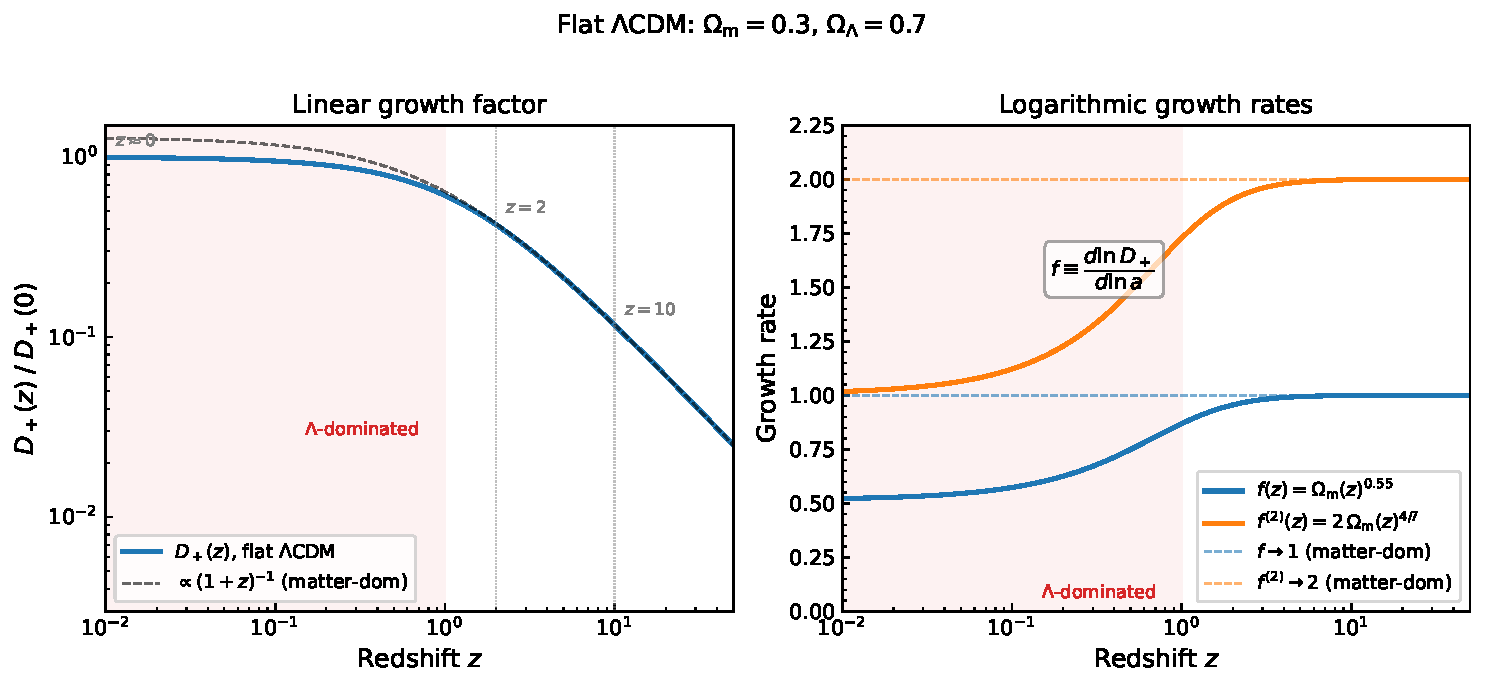
\includegraphics[width=\textwidth]{growth.pdf}
  \caption{Left: linear growth factor $\Dp(z)$ normalized to
  $\Dp(z=0)=1$ for flat $\Lambda$CDM ($\Omm=0.3$, $\Omega_\Lambda=0.7$).
  The dashed line is the matter-domination limit $\Dp \propto (1+z)^{-1}$.
  Right: first-order growth rate $f \approx \Omm(a)^{0.55}$ and
  second-order growth rate $f^{(2)} \approx 2\Omm(a)^{4/7}$.
  Dashed lines show the matter-domination limits $f\to 1$ and
  $f^{(2)}\to 2$.  Both rates decrease at low $z$ as $\Lambda$
  suppresses structure growth.}
  \label{fig:growth}
\end{figure}

%----------------------------------------------------------------------
\section{Lagrangian Perturbation Theory Framework}
\label{sec:lpt}

\subsection{Displacement ansatz}

In comoving coordinates the position of a fluid element initially at
$\bq$ is
%
\begin{equation}
  \bx(\bq, t) = \bq + \bPsi(\bq, t),
  \label{eq:displacement}
\end{equation}
%
where $\bPsi$ is the (comoving) displacement field.  The peculiar
velocity is
%
\begin{equation}
  \bv_{\rm pec} = a\,\dot{\bx} = a\,\dot{\bPsi}.
  \label{eq:vpec_def}
\end{equation}

\subsection{Mass conservation and the Jacobian}

The density field follows from mass conservation.  Each fluid element
initially at $\bq$ carries fixed mass $\bar{\rho}\,d^3q$.  After
displacement it occupies the Eulerian volume element
%
\begin{equation}
  d^3x = \left|\det\!\left(\frac{\partial x_i}{\partial q_j}\right)\right|
          d^3q = |J|\,d^3q,
\end{equation}
%
where $J_{ij} = \partial x_i/\partial q_j$ is the deformation tensor.
Requiring $\rho(\bx)\,d^3x = \bar{\rho}\,d^3q$ gives
$\rho(\bx) = \bar{\rho}/|J|$, so
%
\begin{equation}
  1 + \delta(\bx) \equiv \frac{\rho(\bx)}{\bar{\rho}}
    = \left|\det\!\left(\delta_{ij} +
      \frac{\partial\Psi_i}{\partial q_j}\right)\right|^{-1}
  \equiv |J|^{-1},
  \label{eq:jacobian}
\end{equation}
%
which is \emph{exact} (no perturbative expansion has been made).

\subsection{Perturbative expansion}

In the matter-dominated limit the growing mode scales as $\Dp(t)
\propto a(t)$, and one expands the displacement as a series in
$\Dp$:
%
\begin{equation}
  \bPsi(\bq, t)
    = \Dp(t)\,\bPsi^{(1)}(\bq)
    + \Dpp(t)\,\bPsi^{(2)}(\bq)
    + \cdots,
  \label{eq:lpt_expansion}
\end{equation}
%
where $\Dpp \approx -\tfrac{3}{7}\Dp^2$ in $\Lambda$CDM (exact only in
matter domination; see \S\ref{sec:2lpt_growth}).

%----------------------------------------------------------------------
\section{First Order: the Zel'dovich Approximation}
\label{sec:za}

\subsection{Displacement field}

At first order, the displacement is the gradient of a scalar potential
$\phi^{(1)}$:
%
\begin{equation}
  \bPsi^{(1)}(\bq) = -\nabla_\bq\phi^{(1)}(\bq),
  \label{eq:psi1}
\end{equation}
%
with $\phi^{(1)}$ satisfying the Poisson equation in Lagrangian space:
%
\begin{equation}
  \nabla_\bq^2\phi^{(1)}(\bq) = \delta_{\rm lin}(\bq),
  \label{eq:poisson1}
\end{equation}
%
where $\delta_{\rm lin}$ is the linear density contrast at the
reference epoch at which $\Dp = 1$.
To see where Eq.~(\ref{eq:poisson1}) comes from, linearise the exact
mass-conservation condition $1+\delta = |J|^{-1}$
(Eq.~\ref{eq:jacobian}).
At first order, $J_{ij}=\delta_{ij}+\partial\Psi^{(1)}_i/\partial q_j$
and $\det J\approx 1+\nabla_\bq\cdot\bPsi^{(1)}$, so
%
\begin{equation*}
  \delta \;\approx\; -\nabla_\bq\cdot\bPsi^{(1)}.
\end{equation*}
%
Substituting the potential ansatz $\bPsi^{(1)}=-\nabla_\bq\phi^{(1)}$
gives $\delta=\nabla_\bq^2\phi^{(1)}$, which is
Eq.~(\ref{eq:poisson1}). Physically, the displacement divergence
$\nabla\cdot\bPsi$ measures the fractional change in volume of a
Lagrangian fluid element, hence the local density contrast.

In Fourier space this is solved trivially:
%
\begin{equation}
  \boxed{
  \bPsi^{(1)}(\bk) = -\frac{i\bk}{k^2}\,\delta_{\rm lin}(\bk).
  }
  \label{eq:psi1_fourier}
\end{equation}
%
The IC generator draws $\delta_{\rm lin}(\bk)$ from a complex Gaussian with
variance $P_{\rm lin}(k)/V$ per mode%
\footnote{In a periodic box of volume $V$ the allowed wavevectors are
  discrete with spacing $\Delta^3k=(2\pi)^3/V$.  The real-space variance
  is $\sigma^2=\int d^3k/(2\pi)^3\,P(k)\approx\sum_\bk P(k)/V$,
  so each mode contributes $P(k)/V$ to $\sigma^2$ and must therefore
  be drawn with that variance.  Equivalently, with the DFT convention
  $\delta(\bk)=V^{-1}\!\int d^3x\,\delta(\bx)\,e^{-i\bk\cdot\bx}$
  one has $\langle|\delta(\bk)|^2\rangle=P(k)/V$.
  Larger box $\Rightarrow$ denser mode sampling $\Rightarrow$ smaller variance per mode.}
(the CLASS power spectrum), then applies
Eq.~(\ref{eq:psi1_fourier}) to compute particle displacements.

\subsection{Velocity field}

Differentiating Eq.~(\ref{eq:displacement}) with respect to time and
using $\bPsi = \Dp\bPsi^{(1)}$:
%
\begin{align}
  \bv_{\rm pec}^{(1)}
    &= a\,\dot{\Dp}\,\bPsi^{(1)}
     = a\,Hf\Dp\,\bPsi^{(1)}
     = \calH(a)\,f(a)\,\Dp\,\bPsi^{(1)},
  \label{eq:vel1}
\end{align}
%
where $\calH \equiv aH$ is the conformal Hubble parameter and $f$ is
the logarithmic growth rate from Eq.~(\ref{eq:fgrowth}).  At the IC
redshift this is the conversion MUSIC2 applies via
\texttt{cosmo\_vfact} $= \calH f / h$ to convert displacements to
velocities.

\subsection{Density field}

Linearising the Jacobian determinant in Eq.~(\ref{eq:jacobian}),
%
\begin{equation}
  \delta^{(1)}(\bx) \approx -\nabla_\bq\cdot\bPsi^{(1)}
  = \Dp\,\nabla_\bq^2\phi^{(1)}
  = \Dp\,\delta_{\rm lin}(\bq).
\end{equation}
%
At first order the density contrast is simply the linear field scaled
by the growth factor.

\subsection{Relation between the displacement potential and the
  gravitational potential}
\label{sec:phi_Phi}

The displacement potential $\phi^{(1)}$ satisfies
$\nabla^2\phi^{(1)} = \delta_{\rm lin}$.  On the other hand, the
linearised Poisson equation~(\ref{eq:poisson_lin}) gives
$\nabla^2\Phi = \tfrac{3}{2}H^2\Omm\,a^2\,\delta = \tfrac{3}{2}H^2\Omm\,a^2\Dp\,\delta_{\rm lin}$.
Comparing the two:
%
\begin{equation}
  \phi^{(1)}(\bq; z)
    = \frac{2}{3}\,\frac{\Dp(z)^{-1}}{H^2(z)\,\Omm(z)\,a^2}\,\Phi(\bq; z).
  \label{eq:phi_Phi}
\end{equation}
%
In practice, when $\Phi$ is evaluated at the same epoch as $\Dp$ (so
$\delta = \Dp\delta_{\rm lin}$ with the normalization
$\Phi = \frac{3}{2}H^2\Omm a^2\Dp\phi^{(1)}$), the factor $\Dp^{-1}$
cancels and the relation simplifies to
%
\begin{equation}
  \phi^{(1)}(\bq)
    = \frac{2}{3}\,\frac{1}{H^2(z)\,\Omm(z)\,a^2}\,\Phi(\bq; z),
  \label{eq:phi_Phi_simple}
\end{equation}
%
where $\phi^{(1)}(\bq)$ is the reference-epoch potential (at $\Dp=1$).
Substituting Eqs.~(\ref{eq:psi1}) and (\ref{eq:phi_Phi_simple}) into
Eq.~(\ref{eq:vel1}), the first-order peculiar velocity can be written
directly in terms of the proper gravitational potential:
%
\begin{equation}
  \bv_{\rm pec}^{(1)}(\bq; z)
    = -\frac{2}{3}\,\frac{f(z)}{a\,H(z)\,\Omm(z)}\,
      \nabla_\bq\Phi(\bq; z).
  \label{eq:vpec_Phi}
\end{equation}
%
This is the starting point for linear-theory peculiar-velocity
statistics.

\subsection{Shell crossing and the Zel'dovich pancake}
\label{sec:pancake}

The deformation tensor $\partial\Psi^{(1)}_i/\partial q_j$ is
symmetric in the irrotational case and can therefore be diagonalised
at each point $\bq$.  Denote its eigenvalues by $-\alpha \leq -\beta
\leq -\gamma$ (with $\alpha \geq \beta \geq \gamma$).  The Jacobian
decomposes as
%
\begin{equation}
  J = (1 - \Dp\alpha)(1 - \Dp\beta)(1 - \Dp\gamma),
  \label{eq:J_eigen}
\end{equation}
%
and the Eulerian density along the principal axes is
%
\begin{equation}
  1 + \delta = \frac{1}{J}
    = \frac{1}{(1-\Dp\alpha)(1-\Dp\beta)(1-\Dp\gamma)}.
  \label{eq:delta_eigen}
\end{equation}
%
\emph{Shell crossing} occurs when $J\to 0$, i.e.\ when the largest
eigenvalue satisfies $\Dp\,\alpha = 1$.  Since collapse first occurs
along the direction of largest compression, the first structure to
form is a \emph{pancake}: a flattened sheet perpendicular to the
eigenvector of $\alpha$.  As $\Dp$ grows further, $\Dp\beta=1$ and
$\Dp\gamma=1$ are reached in succession, producing first filaments
then point-like (halo) collapses.

The ZA extends particles through the caustic without stopping them:
once $J<0$ the single-stream assumption breaks down and the density
formula~(\ref{eq:delta_eigen}) is no longer valid.  Higher-order LPT
improves the pre-caustic accuracy but does not cure shell crossing.
ICs must therefore be initialised at sufficiently high redshift that
$\Dp(z_{\rm start})\,\alpha_{\max} < 1$ on all resolved scales.

Figure~\ref{fig:pancake} illustrates this for the simplest case of a
\emph{plane-wave} perturbation $\delta_{\rm lin}(q) = \cos q$, giving
$\Psi^{(1)}(q) = -\sin q$ and $x(q) = q - \Dp\sin q$.  The density
$1+\delta = 1/|1 - \Dp\cos q|$ diverges at the caustic ($\Dp = 1$);
for $\Dp > 1$ the Eulerian map becomes multi-valued (three streams
near $x=0$).  The dashed and dotted curves for $\Dp = 1.2$ show the
regions where $J < 0$ (unphysical in single-stream theory).

\begin{figure}[!t]
  \centering
  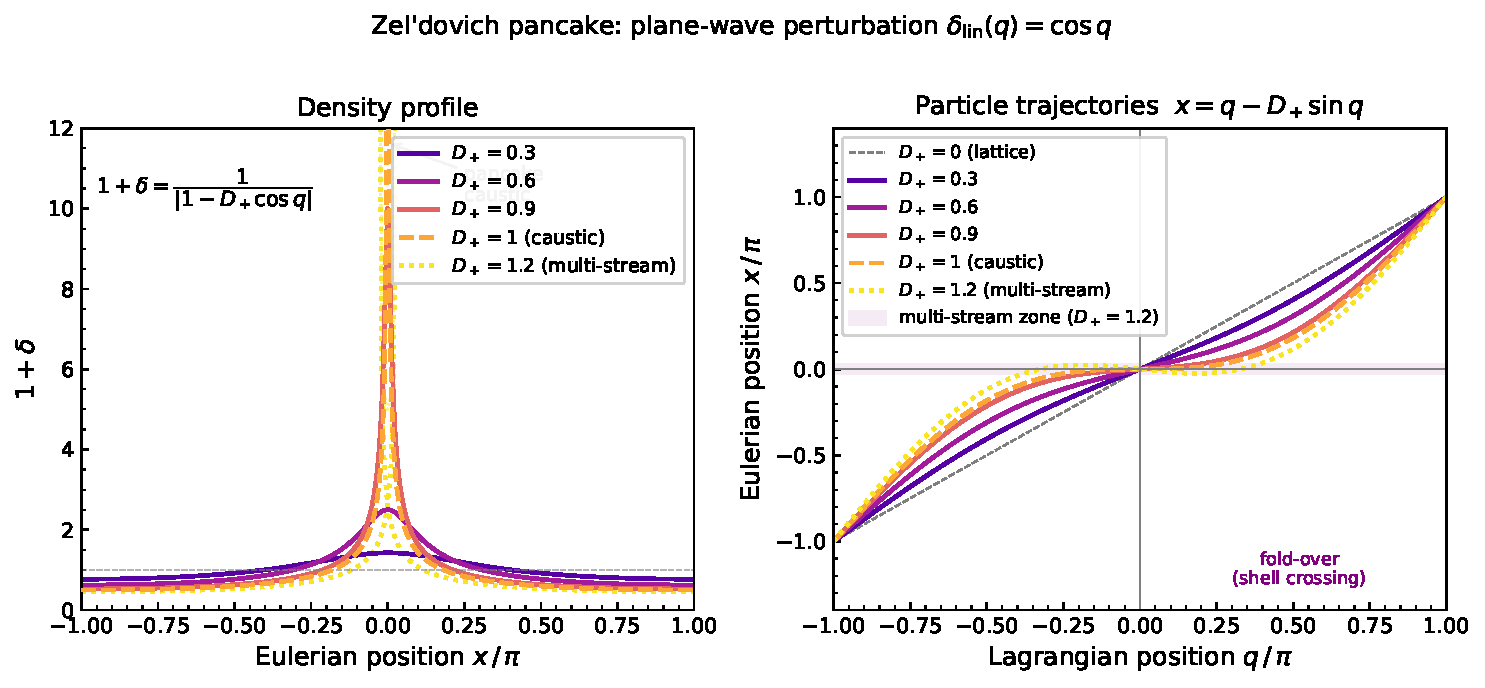
\includegraphics[width=\textwidth]{pancake.pdf}
  \caption{Zel'dovich pancake: plane-wave perturbation
  $\delta_{\rm lin}(q) = \cos q$.
  \textit{Left}: density profile $1+\delta = 1/|1-\Dp\cos q|$ as a
  function of Eulerian position $x$, at several values of the growth
  factor $\Dp$.  The density diverges at $\Dp = 1$ (caustic).  For
  $\Dp = 1.2$ the solid curve shows the physical single-stream region
  ($J>0$) and the dotted continuation is the unphysical multi-stream
  interior.
  \textit{Right}: particle trajectories $x(q) = q - \Dp\sin q$.  For
  $\Dp > 1$ the map folds back at $|q| = \arccos(1/\Dp)$, creating
  a purple-shaded multi-stream zone.  Collapse first occurs along
  the direction of largest eigenvalue $\alpha$, producing a
  flattened sheet (pancake).}
  \label{fig:pancake}
\end{figure}

\subsection{Spherical collapse and the halo threshold $\delta_c$}
\label{sec:spherical}

The Zel'dovich pancake ($\alpha>\beta=\gamma=0$) is one extreme
of the deformation tensor: collapse along a single axis gives a
sheet.  The opposite extreme is \emph{isotropic} compression
$\alpha=\beta=\gamma$, a spherical overdensity, which forms a
point-like halo.  This is the worst-case geometry for IC errors
because the second-order correction is largest when all three
eigenvalues coincide (\S\ref{sec:tophat_timing}).

Consider a uniform spherical overdensity of initial radius $R_i$ and
density $\rho_i=\bar\rho_i(1+\delta_i)$ embedded in an EdS background.
By Birkhoff's theorem the interior evolves as a closed mini-universe
with energy per unit mass
$E=\tfrac{1}{2}\dot r^2-GM/r<0$, $M=\tfrac{4\pi}{3}\bar\rho_i R_i^3(1+\delta_i)$.
The solution is cycloidal
\citep[e.g.][\S3.3]{Tong2019}:
%
\begin{equation}
  r(\tilde\tau)=A(1-\cos\tilde\tau),\qquad
  t(\tilde\tau)=B(\tilde\tau-\sin\tilde\tau),
  \qquad A^3=GMB^2.
  \label{eq:sphcollapse}
\end{equation}
%
Three milestones matter:
\begin{itemize}
  \item \textbf{Turn-around} ($\tilde\tau=\pi$): the sphere reaches
    its maximum radius $r_{\rm ta}=2A$ at $t_{\rm ta}=\pi B$.  The
    actual over-density is
    $\delta(t_{\rm ta})=9\pi^2/16-1\approx 4.55$, while the
    \emph{linear-extrapolated} value is
    $\delta_{\rm lin}(t_{\rm ta})=(3/20)(6\pi)^{2/3}\approx 1.062$.
  \item \textbf{Collapse to a point} ($\tilde\tau=2\pi$): $r\to0$,
    so the actual density diverges.  Linear extrapolation, on the
    other hand, is finite and gives the famous threshold
    %
    \begin{equation}
      \boxed{\;
        \delta_c \;\equiv\; \delta_{\rm lin}(t_{\rm col})
        = \frac{3}{20}(12\pi)^{2/3}
        \;\approx\; 1.686.
      \;}
      \label{eq:deltac}
    \end{equation}
    %
    Any region whose smoothed linear density exceeds $\delta_c$
    today should have already collapsed into a virialised halo.
  \item \textbf{Virialisation}: before reaching the singularity the
    shells shell-cross and redistribute energy until the virial
    theorem is satisfied, $2T+V=0$, giving $r_{\rm vir}=r_{\rm ta}/2$.
    The average density inside $r_{\rm vir}$ relative to the
    background at that time is
    %
    \begin{equation}
      \Delta_{\rm vir}\equiv
      \frac{\rho(r_{\rm vir})}{\bar\rho(t_{\rm col})}
      = 18\pi^2-1 \approx 177,
      \label{eq:Delta_vir}
    \end{equation}
    %
    the origin of the $\rho/\bar\rho=200$ definition used in
    $R_{200}$, $M_{200}$.  In $\Lambda$CDM the number is closer to
    $\Delta_{\rm vir}\approx100$--$200$ depending on $\Omm(z)$
    \citep{Bryan1998}.
\end{itemize}

The threshold $\delta_c\approx 1.686$ is the \emph{linear}
extrapolation of full non-linear collapse --- a point peaks with
$\delta_{\rm lin}\!\ge\!\delta_c$ in the smoothed density field
should be identified with collapsed halos today.
Combined with the variance $\sigma(R)$ of \S\ref{sec:sigma8},
this underlies the Press--Schechter and excursion-set halo mass
functions.

For IC generation the practical message is:
(i) the spherical top-hat is the worst case for ZA-vs-2LPT
accuracy because it saturates the bound
$\delta^{(2)}\le\tfrac{1}{2}|\delta^{(1)}|$
(\S\ref{sec:tophat_timing});
(ii) $\delta_c\approx 1.69$ converts the measured
$\sigma_8(z)$ into a typical collapse redshift, which in turn
determines a safe $z_{\rm start}$: by $z_{\rm start}\gg 1/\sigma_8(0)$
no mode has yet collapsed, validating the perturbative expansion.

%----------------------------------------------------------------------
\section{Second Order: 2LPT}
\label{sec:2lpt}

\subsection{Deriving the second-order source}
\label{sec:2lpt_derive}

To find the second-order displacement, expand the Jacobian
determinant in Eq.~(\ref{eq:jacobian}) in powers of $\bPsi$.
Writing $J_{ij} = \delta_{ij} + \Psi_{i,j}$ and using the identity
$\det(1+\epsilon M) = 1 + \epsilon\,\mathrm{tr}M +
\tfrac{1}{2}\epsilon^2[(\mathrm{tr}M)^2 - \mathrm{tr}(M^2)] +
\mathcal{O}(\epsilon^3)$, we get
%
\begin{equation}
  J = 1
    + \underbrace{\Psi_{i,i}^{(1)}}_{J^{(1)}}
    + \underbrace{\Psi_{i,i}^{(2)}
      + \tfrac{1}{2}\bigl[(\Psi_{i,i}^{(1)})^2
        - \Psi_{i,j}^{(1)}\Psi_{j,i}^{(1)}\bigr]}_{J^{(2)}}
    + \cdots,
  \label{eq:J_expand}
\end{equation}
%
where commas denote partial derivatives with respect to Lagrangian
coordinates $q_j$, and repeated indices are summed.  Mass
conservation requires $\rho\,dV = \bar\rho\,dV_q$, i.e.\
$1+\delta = J^{-1} \approx 1 - J^{(1)} - J^{(2)} + (J^{(1)})^2 + \cdots$.
At first order, $\delta^{(1)} = -\Psi^{(1)}_{i,i} = \nabla^2_\bq\phi^{(1)} = \delta_{\rm lin}$,
as expected.  At second order the equation of motion yields a
sourced Poisson equation for the second-order potential
$\phi^{(2)}$, whose source is precisely the quadratic part:
%
\begin{equation}
  \tfrac{1}{2}\bigl[(\Psi^{(1)}_{i,i})^2
    - \Psi^{(1)}_{i,j}\Psi^{(1)}_{j,i}\bigr]
  = \sum_{i<j}
    \left[\phi^{(1)}_{,ii}\phi^{(1)}_{,jj}
          - \bigl(\phi^{(1)}_{,ij}\bigr)^2\right],
  \label{eq:source_id}
\end{equation}
%
which is the sum of $2\!\times\!2$ minors of the Hessian of
$\phi^{(1)}$, measuring the coupling between different tidal
components.

\subsection{Second-order displacement}

Expanding the equations of motion to second order yields an additional
irrotational displacement
%
\begin{equation}
  \bPsi^{(2)}(\bq) = -\nabla_\bq\phi^{(2)}(\bq),
  \label{eq:psi2}
\end{equation}
%
where the source of $\phi^{(2)}$ is quadratic in the first-order
potential:
%
\begin{equation}
  \boxed{
  \nabla_\bq^2\phi^{(2)}(\bq)
    = \sum_{i < j}
      \left[
        \frac{\partial^2\phi^{(1)}}{\partial q_i^2}
        \frac{\partial^2\phi^{(1)}}{\partial q_j^2}
        -
        \left(\frac{\partial^2\phi^{(1)}}{\partial q_i\,\partial q_j}\right)^{\!2}
      \right].
  }
  \label{eq:poisson2}
\end{equation}
%
The right-hand side is the sum of $2\times 2$ minors of the Hessian
of $\phi^{(1)}$, measuring the coupling between different components
of the tidal field.  In Fourier space this is a mode-coupling integral
(convolution), so $\bPsi^{(2)}$ mixes modes that are independent at
first order.

\subsection{Growth factor at second order}
\label{sec:2lpt_growth}

The second-order growing mode satisfies a separate ODE.  In the
matter-dominated ($\Omm = 1$) limit $\Dpp = -\tfrac{3}{7}\Dp^2$
exactly.  For $\Lambda$CDM a fitting formula accurate to
$\lesssim 0.3\%$ is \citep{Crocce2006}
%
\begin{equation}
  \Dpp(a) \approx -\frac{3}{7}\,\Dp^2(a)\,\Omm(a)^{-1/143}.
  \label{eq:D2}
\end{equation}
%
The corresponding logarithmic growth rate
$f^{(2)} \equiv d\ln|\Dpp|/d\ln a$ is well approximated by
\citep{Bouchet1995}
%
\begin{equation}
  f^{(2)}(a) \approx 2\,\Omm(a)^{4/7},
  \label{eq:f2}
\end{equation}
%
where $\Omm(a)$ is given by Eq.~(\ref{eq:Omm_a}).  In matter
domination $\Omm\to 1$ so $f^{(2)}\to 2$, exactly twice the
first-order rate $f\to 1$.  The 2LPT velocity correction is
%
\begin{equation}
  \bv_{\rm pec}^{(2)}
    = \calH(a)\,f^{(2)}(a)\,\Dpp\,\bPsi^{(2)}.
  \label{eq:vel2}
\end{equation}

\subsection{Total displacement and velocity}

Combining both orders:
%
\begin{align}
  \bx &= \bq + \Dp\,\bPsi^{(1)} + \Dpp\,\bPsi^{(2)},
  \label{eq:x_total}\\
  \bv_{\rm pec} &= \calH(a)\bigl(f\,\Dp\,\bPsi^{(1)}
                   + f^{(2)}\Dpp\,\bPsi^{(2)}\bigr).
  \label{eq:v_total}
\end{align}
%
The generalisation of Eq.~(\ref{eq:vpec_Phi}) to 2LPT is
%
\begin{equation}
  \bv_{\rm pec}(\bq; z)
    = -\frac{2}{3}\,\frac{1}{a\,H(z)\,\Omm(z)}\,
      \sum_{n=1}^{2} f^{(n)}(z)\,\nabla_\bq\Phi^{(n)}(\bq; z),
  \label{eq:vpec_2lpt}
\end{equation}
%
where $\Phi^{(n)}$ is the $n$-th-order proper gravitational potential
and $f^{(1)} \equiv f$.  In MUSIC2 the factor
$(6/7)/v_{\rm fac2lpt}$ in \texttt{main.cc} implements the ratio
$\Dpp/\Dp^2 = -3/7$ and the corresponding velocity coefficient.

%----------------------------------------------------------------------
\section{IC Generation Procedure}
\label{sec:icgen}

Given a linear power spectrum $P_{\rm lin}(k)$ from CLASS and a box
of side $L$ sampled on an $N^3$ grid, the standard FFT-based algorithm
for generating 2LPT initial conditions proceeds as follows
\citep{Jeong2010}.

\subsection{First-order (ZA) step}

\begin{enumerate}
  \item \textbf{Draw the density field.}  For each Fourier mode
    $\bk = (2\pi/L)\,\mathbf{n}$ with $|\mathbf{n}| \leq N/2$,
    draw a complex Gaussian random number $\delta_{\rm lin}(\bk)$
    with variance $\langle|\delta_{\rm lin}(\bk)|^2\rangle =
    P_{\rm lin}(k)/V$ (where $V=L^3$).  Enforce the Hermitian
    condition $\delta_{\rm lin}(-\bk)=\delta_{\rm lin}^*(\bk)$ so
    that the real-space field is real (see Appendix~\ref{app:fft}).
    An optional fixed-amplitude mode is discussed in the box below.

  \item \textbf{Compute the first-order potential.}  In Fourier space,
    Eq.~(\ref{eq:poisson1}) is trivially inverted:
    %
    \begin{equation}
      \phi^{(1)}(\bk) = -\frac{\delta_{\rm lin}(\bk)}{k^2}.
      \label{eq:phi1_fourier}
    \end{equation}

  \item \textbf{Compute the displacement components.}  The six
    second-derivative fields $\phi^{(1)}_{,ij}$ needed for the
    source (Eq.~\ref{eq:poisson2}) are obtained by multiplying
    $\phi^{(1)}(\bk)$ by $-k_ik_j$ in Fourier space and
    transforming back.  The three displacement components are
    $\Psi^{(1)}_i(\bk) = ik_i\phi^{(1)}(\bk)$, each obtained by
    a single IFFT.
\end{enumerate}

% ---------------------------------------------------------------------------
\begin{tcolorbox}[
  title={Fixed-amplitude (``paired-and-fixed'') ICs \citep{Angulo2016}},
  colback=gray!5,
  colframe=gray!55!black,
  coltitle=white,
  fonttitle=\bfseries,
  breakable,
  before skip=1.2em,
  after skip=1.2em
]

\textbf{Standard draw and cosmic variance.}
In the standard algorithm the real and imaginary parts of each mode are drawn
independently,
$\mathrm{Re}[\delta(\bk)],\,\mathrm{Im}[\delta(\bk)]
 \sim \mathcal{N}(0,\,P(k)/2V)$.
The amplitude $|\delta(\bk)|$ therefore follows a \emph{Rayleigh
distribution} — it is the magnitude of a 2D Gaussian vector — and the
power per mode $|\delta(\bk)|^2$ is exponentially distributed with mean
$P(k)/V$ and 100\,\% fractional scatter.
Averaging $N_k$ independent modes in a wavenumber bin yields the estimator
$\hat{P}(k) = (V/N_k)\sum_{|\bk|\approx k}|\delta(\bk)|^2$ with cosmic
variance
%
\begin{equation*}
  \frac{\sigma[\hat{P}(k)]}{P(k)} \simeq \sqrt{\frac{2}{N_k}}.
\end{equation*}

\textbf{Fixed-amplitude technique.}
\citet{Angulo2016} proposed replacing the Rayleigh draw with a deterministic
amplitude $|\delta(\bk)| = \sqrt{P(k)/V}$ exactly, while keeping the
phase $\theta_\bk \sim \mathrm{Uniform}[0,2\pi)$ random.
Each mode now matches the target power spectrum precisely, so
$\hat{P}(k) = P(k)$ mode-by-mode and the amplitude contribution to
cosmic variance is eliminated.
MUSIC2 implements this via \texttt{fix\_mode\_amplitude = yes}
(the default in this pipeline).

\textbf{Paired simulations.}
A complementary technique is to generate a \emph{partner} IC with
$\delta'(\bk) = -\delta(\bk)$, i.e.\ all phases shifted by $\pi$, which
in real space gives $\delta'(\bx) = -\delta(\bx)$.
For any observable $f$ that admits a perturbative expansion in $\delta$,
%
\begin{equation*}
  \frac{f[\delta]+f[-\delta]}{2}
  = f^{(0)} + f^{(2)}[\delta,\delta] + f^{(4)}[\delta,\delta,\delta,\delta]
  + \cdots
\end{equation*}
%
all odd-order contributions cancel exactly.
Because sample variance is dominated by the linear term $f^{(1)}$,
averaging a pair of simulations dramatically reduces cosmic variance
for two-point statistics ($P(k)$, $\xi(r)$, $\sigma_8$).
The fixed-amplitude and pairing techniques are independent and can be
combined for maximum variance suppression.

\textbf{Why the field is no longer Gaussian.}
A Gaussian random field (GRF) requires that the real and imaginary parts of
every mode are \emph{independently} Gaussian-distributed, so $|\delta(\bk)|$
must be free to fluctuate (Rayleigh-distributed).
Fixing $|\delta(\bk)|$ to a constant removes this degree of freedom:
the joint distribution of all modes is no longer multivariate Gaussian.
In real space, the one-point PDF of $\delta(\bx)$ still looks approximately
Gaussian (central limit theorem over many modes), but higher-order connected
correlators such as the bispectrum $\langle\delta\delta\delta\rangle_c$ and
trispectrum $\langle\delta\delta\delta\delta\rangle_c$ are suppressed
relative to a true GRF.
Fixed-amplitude ICs are therefore \emph{unsuitable} for studies of primordial
non-Gaussianity ($f_{\rm NL}$) or any statistic sensitive to higher-order
correlations.
\end{tcolorbox}

\subsection{Second-order step}

\begin{enumerate}
  \item \textbf{Build the source in real space.}  From the six
    real-space fields $\phi^{(1)}_{,ij}(\bq)$ obtained above,
    compute
    %
    \begin{equation}
      F(\bq) = \sum_{i<j}
        \Bigl[\phi^{(1)}_{,ii}(\bq)\,\phi^{(1)}_{,jj}(\bq)
              - \bigl(\phi^{(1)}_{,ij}(\bq)\bigr)^2\Bigr].
      \label{eq:F_source}
    \end{equation}
    %
    This requires no additional FFTs once the $\phi^{(1)}_{,ij}$
    fields are available.

  \item \textbf{Solve for $\phi^{(2)}$.}  FFT $F(\bq)$ to Fourier
    space and divide by $-k^2$:
    %
    \begin{equation}
      \phi^{(2)}(\bk) = -\frac{F(\bk)}{k^2}.
      \label{eq:phi2_fourier}
    \end{equation}
    %
    The $\Omm^{-1/143}$ correction (Eq.~\ref{eq:D2}) is applied
    when multiplying by the growth factor $\Dpp$.

  \item \textbf{Compute $\bPsi^{(2)}$.}  Multiply by $i\bk$ in
    Fourier space and IFFT to get the three components of
    $\bPsi^{(2)}(\bq) = -\nabla_\bq\phi^{(2)}(\bq)$.
\end{enumerate}

\subsection{Assigning positions and velocities}

At redshift $z_{\rm start}$ (scale factor $a$), the particle
positions and peculiar velocities are:
%
\begin{align}
  \bx &= \bq
       + \Dp(z)\,\bPsi^{(1)}(\bq)
       + \Dpp(z)\,\bPsi^{(2)}(\bq),
  \label{eq:x_ic}\\[4pt]
  \bv_{\rm pec} &= \calH(a)\Bigl[
       f(z)\,\Dp(z)\,\bPsi^{(1)}(\bq)
     + f^{(2)}(z)\,\Dpp(z)\,\bPsi^{(2)}(\bq)\Bigr],
  \label{eq:v_ic}
\end{align}
%
where $\calH = aH$ is the conformal Hubble parameter,
$f \approx \Omm(z)^{0.55}$ (Eq.~\ref{eq:fgrowth}) and
$f^{(2)} \approx 2\Omm(z)^{4/7}$ (Eq.~\ref{eq:f2}).
SWIFT stores $\bv_{\rm int} = a\,\bv_{\rm pec}$, so the stored
quantity is $\calH(f\Dp\bPsi^{(1)} + f^{(2)}\Dpp\bPsi^{(2)})$.

Figure~\ref{fig:icgen} summarises the complete 2LPT algorithm as
a flowchart.

\begin{figure}[!t]
\centering
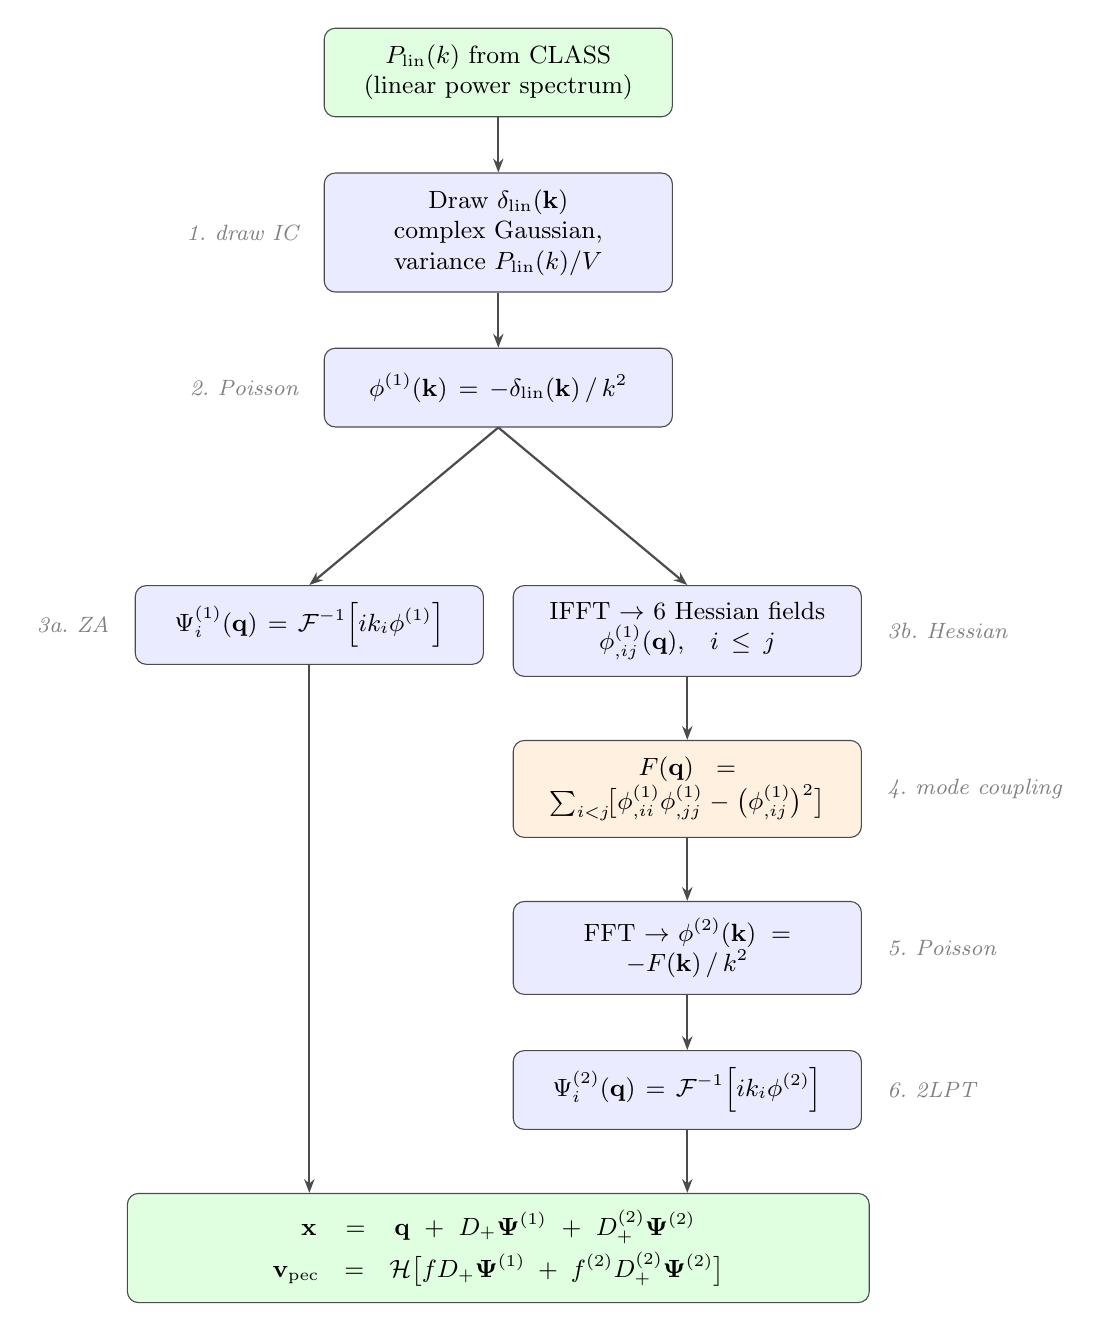
\begin{tikzpicture}[
  box/.style  = {rectangle, rounded corners=4pt, draw=black!70,
                 fill=#1, text width=4.0cm, align=center,
                 font=\small, inner sep=6pt, minimum height=1.0cm},
  box/.default = blue!8,
  arrow/.style = {-{Stealth[length=5pt]}, thick, black!70},
  label/.style = {font=\footnotesize\itshape, text=gray}
]

%% ─── Shared top chain (centred) ─────────────────────────────────
\node[box=green!12] (input)
  {$P_{\rm lin}(k)$ from CLASS\\(linear power spectrum)};

\node[box, below=0.7cm of input] (draw)
  {Draw $\delta_{\rm lin}(\bk)$\\complex Gaussian,\\
   variance $P_{\rm lin}(k)/V$};

\node[box, below=0.7cm of draw] (phi1k)
  {$\phi^{(1)}(\bk) = -\delta_{\rm lin}(\bk)\,/\,k^2$};

%% ─── Left branch (ZA): Ψ^(1) ────────────────────────────────────
\node[box, below=2.0cm of phi1k, xshift=-2.4cm] (psi1)
  {$\Psi^{(1)}_i(\bq) = \mathcal{F}^{-1}\!\left[ik_i\phi^{(1)}\right]$};

%% ─── Right branch (2LPT): Hessian → F → φ^(2) → Ψ^(2) ──────────
\node[box, below=2.0cm of phi1k, xshift=2.4cm] (hess)
  {IFFT $\to$ 6 Hessian fields\\
   $\phi^{(1)}_{,ij}(\bq)$,\quad $i\!\leq\! j$};

\node[box=orange!12, below=0.8cm of hess] (source)
  {$F(\bq) = \!\sum_{i<j}\!\bigl[
     \phi^{(1)}_{,ii}\phi^{(1)}_{,jj}
     - \bigl(\phi^{(1)}_{,ij}\bigr)^{2}\bigr]$};

\node[box, below=0.8cm of source] (phi2k)
  {FFT $\to$ $\phi^{(2)}(\bk) = -F(\bk)\,/\,k^2$};

\node[box, below=0.7cm of phi2k] (psi2)
  {$\Psi^{(2)}_i(\bq) = \mathcal{F}^{-1}\!\left[ik_i\phi^{(2)}\right]$};

%% ─── Final: assign positions + velocities (centred) ─────────────
\node[box=green!12,
      below=0.8cm of psi2, xshift=-2.4cm,  %% centres below phi1k
      text width=9.0cm] (final)
  {$\bx = \bq + \Dp\bPsi^{(1)} + \Dpp\bPsi^{(2)}$\\[2pt]
   $\bv_{\rm pec} = \calH\bigl[f\Dp\bPsi^{(1)}
     + f^{(2)}\Dpp\bPsi^{(2)}\bigr]$};

%% ─── Arrows: shared stem ────────────────────────────────────────
\draw[arrow] (input)  -- (draw);
\draw[arrow] (draw)   -- (phi1k);

%% ─── Fork: diagonal arrows from φ^(1) to each branch ───────────
\draw[arrow] (phi1k.south) -- (psi1.north);
\draw[arrow] (phi1k.south) -- (hess.north);

%% ─── Arrows: right branch ───────────────────────────────────────
\draw[arrow] (hess)   -- (source);
\draw[arrow] (source) -- (phi2k);
\draw[arrow] (phi2k)  -- (psi2);

%% ─── Merge arrows → final (straight down into wide box) ─────────
\draw[arrow] (psi1.south) -- (final.north -| psi1);
\draw[arrow] (psi2.south) -- (final.north -| psi2);

%% ─── Step labels ────────────────────────────────────────────────
\node[label, left=0.2cm of draw,    anchor=east] {1.~draw IC};
\node[label, left=0.2cm of phi1k,   anchor=east] {2.~Poisson};
\node[label, left=0.2cm of psi1,    anchor=east] {3a.~ZA};
\node[label, right=0.2cm of hess,   anchor=west] {3b.~Hessian};
\node[label, right=0.2cm of source, anchor=west] {4.~mode coupling};
\node[label, right=0.2cm of phi2k,  anchor=west] {5.~Poisson};
\node[label, right=0.2cm of psi2,   anchor=west] {6.~2LPT};

\end{tikzpicture}
\caption{Flowchart of the 2LPT IC generation algorithm
(\S\ref{sec:icgen}).  Green boxes are inputs/outputs; blue boxes are
computational steps; the orange box is the second-order source.
After solving the first-order Poisson equation for $\phi^{(1)}(\bk)$,
the algorithm forks into two parallel branches (3a and 3b):
the left branch computes the ZA displacement $\bPsi^{(1)}$ directly
from $\phi^{(1)}$, while the right branch computes six Hessian fields
$\phi^{(1)}_{,ij}(\bq)$ needed for the 2LPT mode-coupling source $F(\bq)$.
The two displacement fields $\bPsi^{(1)}$ and $\bPsi^{(2)}$ are combined
in the final step to assign particle positions and velocities.
All transforms are 3D FFTs.}
\label{fig:icgen}
\end{figure}

%----------------------------------------------------------------------
\section{Starting Redshifts and Convergence}
\label{sec:zstart}

A practical question is: how early must ICs be generated?
\citet{Crocce2006} showed that ZA-only ICs excite decaying modes
that decay only as $a^{-1}$, causing an artificial \emph{suppression}
of power that persists to low redshift.  Concretely, even starting at
$z_{\rm start}=400$, ZA ICs leave a $\sim\!1\%$ power deficit relative
to 2LPT ICs at all $z=1$--6 \citep{Jeong2010}.

2LPT ICs also excite transients (with the opposite sign: a small
\emph{amplification} of power), but these decay much more rapidly
with $a$.  Simulations starting from 2LPT at $z_{\rm start}=300$
agree with those at $z_{\rm start}=400$ to better than $1\%$ at
$z<6$, demonstrating convergence.

\medskip
In summary:
\begin{itemize}
  \item \textbf{ZA}: transients $\propto a^{-1}$; convergence
    requires $z_{\rm start} \gg 1000$, which is impractical.
    At $z_{\rm start}=50$--$400$ a $\sim\!1$--$10\%$ power
    suppression remains at $z \lesssim 6$.
  \item \textbf{2LPT}: transients decay rapidly.
    $z_{\rm start} \gtrsim 50$ gives $<1\%$ error at $z<6$;
    $z_{\rm start} \approx 300$ is effectively converged.
  \item For most IC codes (including \textsc{music2}) using 2LPT
    with $z_{\rm start} \approx 50$--$100$ is standard for
    large-scale structure simulations.
\end{itemize}

\paragraph{Truncation vs.\ discreteness: an unavoidable trade-off.}
Raising $z_{\rm start}$ is not a free parameter to be pushed arbitrarily
high.  Two competing errors set the optimal starting redshift, nicely
reviewed by \citet{Angulo2022} (their \S8.3):
%
\begin{itemize}
  \item \textbf{Truncation error.}  Finite-order LPT is a low-order
    truncation of the full non-linear dynamics, so the density field
    handed to the $N$-body code contains a transient that grows as
    $a^{m+1}$ for $m$-th order LPT (so ZA: $\propto a$, 2LPT:
    $\propto a^2$, 3LPT: $\propto a^3$).  This error is
    \emph{largest at late starting times}, pushing one towards higher
    $z_{\rm start}$.
  \item \textbf{Discreteness error.}  Once an $N$-body code takes over,
    the dynamics are those of a \emph{discrete} system of
    self-gravitating particles on a pre-IC lattice.  The linear
    dispersion relation of the lattice differs from the continuum
    \citep{MarcosEtal2006,Garrison2016}; small force inaccuracies
    (round-off, tree opening, softening transitions) also accumulate
    more aggressively when $\delta$ is tiny and much of the
    gravitational signal sits in the noise.  This error is
    \emph{largest at early starting times}, pushing one towards lower
    $z_{\rm start}$.
\end{itemize}
%
The sweet spot depends on the LPT order, the pre-IC lattice, and the
target accuracy.  \citet{Michaux2020} showed that 3LPT combined with a
BCC or FCC load and a relatively late start ($z_{\rm start} \sim 11$--$24$)
matches a deep reference run to sub-percent accuracy on $P(k)$ and the
bispectrum up to $k \lesssim 2\,h\,{\rm Mpc}^{-1}$, whereas ZA at the
same $z_{\rm start}$ leaves visible systematic biases (see fig.~23 of
\citealt{Angulo2022} reproduced from \citealt{Michaux2020}).
\citet{RampfHahn2021} further show that LPT converges rapidly before
shell crossing, so for most practical purposes 3LPT is sufficient;
higher orders are needed only in special regimes.  Exclusion of
``corner modes'' ($k > k_{\rm Ny}$, i.e.\ $k$ between $1$ and
$\sqrt{3}\,k_{\rm Ny}$ in the $N^3$ cube) when constructing $n \ge 3$
LPT terms further suppresses UV truncation artefacts from the
convolution integrals, with negligible impact on non-linear results
for $n \le 2$ \citep{RampfHahn2021,Falck2017}.

%----------------------------------------------------------------------
\section{Relation to the Power Spectrum}
\label{sec:pk}

\subsection{Power spectrum and two-point correlation function}
\label{sec:pk_xi}

The \emph{matter power spectrum} $P(k)$ is defined by the two-point
expectation value of the Fourier-space density contrast
\citep[e.g.][Eq.~1.2]{Jeong2010}:
%
\begin{equation}
  \langle \delta(\bk)\,\delta^*(\bk') \rangle
  = (2\pi)^3\,P(k)\,\delta^D(\bk - \bk'),
  \label{eq:pk_def}
\end{equation}
%
where $\delta(\bx) \equiv \rho(\bx)/\bar\rho - 1$ and statistical
isotropy restricts $P$ to depend only on $k = |\bk|$.  In linear
theory $\delta(\bk, z) = \Dp(z)\,\delta_0(\bk)$, so the amplitude
evolves as
%
\begin{equation}
  P(k, z) = \Dp^2(z)\,P(k, 0),
  \label{eq:pk_z}
\end{equation}
%
while the shape is frozen.

The real-space \emph{two-point correlation function}
$\xi(r) \equiv \langle\delta(\bx)\,\delta(\bx+\br)\rangle$ is the
Fourier-space transform pair of $P(k)$.  Exploiting isotropy to reduce
the 3D integral via the spherical Bessel function
$j_0(x) = \sin(x)/x$:
%
\begin{align}
  \xi(r) &= \frac{1}{2\pi^2}\int_0^\infty dk\; k^2\, P(k)\, j_0(kr),
  \label{eq:xi_pk} \\[4pt]
  P(k)   &= 4\pi\int_0^\infty dr\; r^2\, \xi(r)\, j_0(kr).
  \label{eq:pk_xi_inv}
\end{align}
%
Physically, $\xi(r)$ is the excess probability of finding two mass
elements separated by comoving distance $r$ relative to a uniform
distribution.  It is positive where matter is clustered
($r \lesssim 50\,h^{-1}\,\mathrm{Mpc}$ today), crosses zero, and
shows the baryon acoustic oscillation (BAO) peak at
$r_{\rm BAO} \approx 105\,h^{-1}\,\mathrm{Mpc}$.  The two statistics
carry identical information for Gaussian fields; $P(k)$ is the natural
choice for quasi-linear and non-linear scales ($k \gtrsim
0.1\,h\,\mathrm{Mpc}^{-1}$), while $\xi(r)$ is convenient for the
BAO feature in configuration space.

\subsection{Shape of the linear $P(k)$: primordial spectrum and transfer function}
\label{sec:pk_shape}

The linear matter power spectrum factorises into a \emph{primordial}
piece set by inflation and a \emph{transfer function} $T(k)$ that
records how each Fourier mode evolved between horizon re-entry and
matter--radiation equality
\citep[see e.g.][\S3.1--3.2]{Tong2019}:
%
\begin{equation}
  P_{\rm lin}(k, z)
    = A_s\!\left(\frac{k}{k_*}\right)^{\!n_s-1}
      \cdot k\, T^{2}(k)\cdot\Dp^{2}(z).
  \label{eq:pk_shape}
\end{equation}
%
Here $A_s$ is the scalar amplitude of curvature perturbations,
$k_*\sim 0.05\,\mathrm{Mpc}^{-1}$ is a pivot scale, and $n_s\approx
0.965$ is the scalar spectral tilt measured by Planck.

\paragraph{Primordial power spectrum.}
Inflation generates a near scale-invariant curvature spectrum
$\mathcal{P}_\mathcal{R}(k)\propto k^{n_s-1}$.  The
\emph{dimensionless} density power spectrum is
$\Delta^2(k)\equiv k^3 P(k)/(2\pi^2)$, and ``scale invariance'' means
the corresponding gravitational-potential spectrum
$\Delta^2_\Phi(k)\propto k^{-1}\Delta^2(k)$ is flat (via Poisson,
$\Phi\propto\delta/k^2$).  This picks out $P(k)\propto k^{n_s}$ with
$n_s=1$ as the Harrison--Zel'dovich limit.  The small deviation
$n_s-1\approx -0.035$ is a direct signature of the dynamics of
inflation \citep[see][\S3.2.1]{Tong2019}.

\paragraph{Transfer function and the Meszaros effect.}
A mode with comoving wavenumber $k$ enters the Hubble radius when
$k=\calH(a)$.  In matter domination the gravitational source term
and the Hubble friction combine to give growing and decaying modes
$\delta\propto a,\ a^{-3/2}$, so modes that enter in MD grow
unsuppressed.  In the radiation era, however, the dark matter
density contrast $\delta_m$ on sub-horizon scales obeys the
\emph{Meszaros equation} \citep[][\S5.1]{Baumann2022}:
%
\begin{equation}
  \frac{d^2\delta_m}{dy^2}
    + \frac{2+3y}{2y(1+y)}\frac{d\delta_m}{dy}
    - \frac{3}{2y(1+y)}\delta_m = 0,
  \qquad y\equiv a/a_{\rm eq},
  \label{eq:meszaros}
\end{equation}
%
whose growing solution is $\delta_m\propto(2+3y)$: during RD
($y\ll1$) it grows only \emph{logarithmically} in $\ln y$, because
the radiation background is not clustered to provide a gravitational
source.  Sub-horizon DM modes therefore ``stall'' between horizon
entry and equality, while super-horizon modes grow normally.

Define the comoving wavenumber of the horizon at equality,
%
\begin{equation}
  k_{\rm eq} \;\simeq\; 0.07\,\Omm h^2\,\mathrm{Mpc}^{-1}
              \;\approx\; 0.015\,h\,\mathrm{Mpc}^{-1}
  \qquad\text{(Planck cosmology)}.
  \label{eq:keq}
\end{equation}
%
Modes with $k<k_{\rm eq}$ entered the horizon in the matter era and
carry no suppression: $T(k)\to1$.  Modes with $k>k_{\rm eq}$ entered
in RD and stalled for a factor $\sim(a_{\rm enter}/a_{\rm eq})^{2}
=(k_{\rm eq}/k)^2$ in scale factor, giving $T(k)\propto(k_{\rm eq}/k)^2$
at $k\gg k_{\rm eq}$.  Combining with
Eq.~(\ref{eq:pk_shape}) yields the familiar two-limit shape
\citep[\S5.1]{Baumann2022}:
%
\begin{equation}
  P_{\rm lin}(k)\propto
  \begin{cases}
    k^{n_s} \approx k,        & k\ll k_{\rm eq}\\[3pt]
    k^{n_s-4}\approx k^{-3}\ln^2(k/k_{\rm eq}), & k\gg k_{\rm eq}
  \end{cases}
  \label{eq:pk_limits}
\end{equation}
%
with a broad turnover around $k_{\rm eq}$.  The log factor at
$k\gg k_{\rm eq}$ is the residual Meszaros growth in RD.
Accurate fitting formulae (BBKS, \citealt{Jeong2010};
Eisenstein--Hu) exist, but in practice one takes $T(k)$ tabulated
from a Boltzmann code (CLASS, CAMB).

\paragraph{Baryon acoustic oscillations.}
Before decoupling, baryons and photons oscillate as a coupled
plasma; the resulting sound horizon at drag epoch
($r_d\simeq 147\,\mathrm{Mpc}$) imprints small oscillatory features
on $T(k)$ at $k\sim(1$--$4)\times10^{-1}\,h\,\mathrm{Mpc}^{-1}$ with
amplitude $\sim 10\%$ of $\Delta^2(k)$.  They are more visible as
the BAO peak in $\xi(r)$ at $r\approx 105\,h^{-1}\,\mathrm{Mpc}$
(\S\ref{sec:pk_xi}).

\subsection{Variance and $\sigma_8$}
\label{sec:sigma8}

The most common one-number summary of $P(k)$ is the variance of
$\delta$ smoothed on comoving scale $R$.  Let $W_R(\bx)$ be a
spherical filter of characteristic radius $R$ and define the
smoothed field
$\delta_R(\bx)\equiv\int d^3x'\,W_R(\bx-\bx')\,\delta(\bx')$.
By the convolution theorem $\delta_R(\bk)=\tilde W_R(k)\,\delta(\bk)$,
so the real-space variance reduces to a one-dimensional integral over
$P(k)$ \citep[][eq.~2.21]{Jeong2010}:
%
\begin{equation}
  \sigma^2(R,z) = \int\!\frac{d^3k}{(2\pi)^3}\,\tilde W_R^2(k)\,P(k,z)
  = \int_0^\infty\!d\ln k\;\Delta^2(k,z)\,\tilde W_R^2(k).
  \label{eq:sigmaR}
\end{equation}
%
For the spherical top-hat of radius $R$, the Fourier transform is
%
\begin{equation}
  \tilde W_R^{\rm TH}(k)
    = \frac{3[\sin(kR)-kR\cos(kR)]}{(kR)^3}.
  \label{eq:wtop}
\end{equation}
%
The quantity
$\sigma_8\equiv\sigma(R=8\,h^{-1}\,\mathrm{Mpc},\,z=0)$ is the
standard amplitude normalisation: $\sigma_8\approx 0.81$ in Planck
2018.  Because $\Dp(z)$ factorises, $\sigma_8(z)=\sigma_8(0)\Dp(z)$,
and Eq.~(\ref{eq:sigmaR}) at general $R$ is the sum over modes
that fit inside a sphere of radius $R$.  The particular choice
$R=8\,h^{-1}\,\mathrm{Mpc}$ is historical: $\sigma\sim1$ at this
scale today, so it marks the approximate onset of non-linear
clustering.  Larger $\sigma_8$ means structure formation began
earlier \citep[][\S3.2.5]{Tong2019}.

\begin{tcolorbox}[colback=gray!5, colframe=gray!55!black,
                  title={\bfseries Parseval and $\sigma_8$ in one line},
                  coltitle=white, fonttitle=\bfseries,
                  before skip=1em, after skip=1em]
Setting $\tilde W_R=1$ in Eq.~(\ref{eq:sigmaR}) recovers the
\emph{total} variance $\langle\delta^2\rangle$, so $\sigma^2(R)$ is
literally Parseval's theorem applied to the top-hat-smoothed field.
Novices often confuse $\sigma_8$ with ``the amplitude of $P(k)$ at
$k=1/(8\,h^{-1}\,\mathrm{Mpc})$''.  It is not: $\sigma_8$ is an
\emph{integral} over all $k$, weighted by the top-hat window.
Modes at $k\ll 1/R$ contribute via $\tilde W_R\to 1$; modes at
$k\gg 1/R$ are strongly suppressed.
\end{tcolorbox}

\subsection{What CLASS provides}
\label{sec:class_output}

CLASS solves the linearised Einstein--Boltzmann system for
photons, baryons, CDM, neutrinos, and metric perturbations, and
outputs the \emph{linear} matter power spectrum
$P_{\rm lin}(k,z)$ on a user-specified $(k,z)$ grid.
In our pipeline (\texttt{run\_pipeline.sh}) the CLASS output file
\texttt{data/class\_pk\_z\{z\}\_pk.dat} has two columns:
%
\begin{center}
\begin{tabular}{lll}
\hline
Column & Units & Content \\
\hline
$k$     & $[h\,\mathrm{Mpc}^{-1}]$ & comoving wavenumber \\
$P(k)$  & $[(h^{-1}\,\mathrm{Mpc})^{3}]$ & linear matter $P$ at $z=z_{\rm pk}$ \\
\hline
\end{tabular}
\end{center}
%
The $h$ factors reflect CLASS's \texttt{format=class} convention
(which is the MUSIC2 default).  This power spectrum is the correct
input to MUSIC2 (\S\ref{sec:icgen}) and the correct comparison for
the 1LPT (ZA) density field.  Validation against the ICs at high
$z$ requires the back-scaling correction of
\S\ref{sec:backscaling_radiation}.

\begin{tcolorbox}[colback=yellow!5, colframe=orange!50!black,
                  title={\bfseries Fourier-convention pitfall},
                  coltitle=white, fonttitle=\bfseries,
                  before skip=1em, after skip=1em]
CLASS defines $P(k)$ through
$\langle\delta(\bk)\delta^*(\bk')\rangle
 =(2\pi)^3 P(k)\,\delta^D(\bk-\bk')$
with $\delta(\bk)=\int d^3x\,\delta(\bx)\,e^{-i\bk\cdot\bx}$
(forward transform \emph{without} a $(2\pi)^{-3}$ prefactor).
This is the ``physicist's / Peebles convention''
(Appendix~\ref{app:fft}; \citealt{Jeong2010}, App.~A).  Codes in
engineering or signal-processing conventions place the
$(2\pi)^{-3}$ differently and require a rescaling of the CLASS
output before use.  \emph{No rescaling is needed anywhere in this
pipeline} --- MUSIC2, \texttt{compute\_pk.py}, and CLASS all use
the same convention.
\end{tcolorbox}

\subsection{Non-linear corrections from 2LPT}

Because the 2LPT displacement is quadratic in $\delta_{\rm lin}$, the
resulting density field contains contributions at second order in
$\delta_{\rm lin}$.  At one loop, the power spectrum of the displaced
particle distribution is \citep{Bernardeau2002}
%
\begin{equation}
  P_{\rm 2LPT}(k)
    = P_{\rm lin}(k)
    + P_{22}(k)
    + 2\,P_{13}(k)
    + \mathcal{O}(\delta_{\rm lin}^6),
  \label{eq:pk_loop}
\end{equation}
%
where the one-loop terms involve convolutions of $P_{\rm lin}$:
%
\begin{align}
  P_{22}(k) &= 2\int\!\frac{d^3q}{(2\pi)^3}\,
    \left[F_2(\bk-\mathbf{q},\,\mathbf{q})\right]^2
    P_{\rm lin}(|\bk-\mathbf{q}|)\,P_{\rm lin}(q), \\
  P_{13}(k) &= 3\,P_{\rm lin}(k)\int\!\frac{d^3q}{(2\pi)^3}\,
    F_3(\bk,\mathbf{q},-\mathbf{q})\,P_{\rm lin}(q),
\end{align}
%
with $F_2$, $F_3$ the standard perturbation theory (SPT) mode-coupling
kernels.  Consequently the power spectrum measured from the IC
particles will lie \emph{above} the CLASS linear theory at high $k$,
even before any non-linear evolution.

\subsection{Size of the correction}

The one-loop terms scale as $P_{\rm lin}^2 \propto \sigma_8^4(z)$.
Since $\sigma_8(z) = \sigma_8(0)\,\Dp(z)$ and $\Dp(z) \approx
1/(1+z)$ in matter domination:
%
\begin{equation}
  \frac{P_{22}+2P_{13}}{P_{\rm lin}} \sim \sigma_8^2(z)
    = \left[\frac{\sigma_8(0)}{1+z}\right]^2.
\end{equation}
%
For our CV\_22 cosmology ($\sigma_8 = 0.8$):
%
\begin{center}
\begin{tabular}{lcc}
\hline
Redshift & $\sigma_8(z)$ & One-loop correction \\
\hline
$z = 127$ & 0.006 & $\lesssim 0.004\%$ \\
$z = 45$  & 0.017 & $\lesssim 0.03\%$  \\
$z = 2$   & 0.27  & $\sim 7\%$ (high $k$) \\
$z = 0.5$ & 0.55  & $\sim 30\%$ (high $k$) \\
\hline
\end{tabular}
\end{center}
%
For $z \gtrsim 10$ the linear approximation is excellent.  At $z = 2$
(our default pipeline redshift) deviations are visible at $k \gtrsim
0.5\,h\,\mathrm{Mpc}^{-1}$.  A consistent comparison at $z \lesssim 5$
requires a one-loop prediction from a code such as \textsc{PyBird},
\textsc{velocileptors}, or CLASS with \texttt{halofit}.

%----------------------------------------------------------------------
\section{Why 2LPT Matters for ICs}
\label{sec:why2lpt}

\subsection{Transients from ZA initial conditions}

ZA sets the second-order displacement $\bPsi^{(2)}$ to zero, so the
initial particle distribution is misplaced relative to the exact
second-order solution.  The $N$-body gravity then has to supply the
missing $\bPsi^{(2)}$ as the simulation evolves.  During this
``catch-up'' phase, spurious mode-coupling terms are excited that
decay only as $a^{-1}$ \citep{Crocce2006} — taking many dynamical
times to die away and leaving a residual suppression of power at
$z \lesssim 6$ even when starting at $z_{\rm start}=400$.
2LPT encodes $\bPsi^{(2)}$ in the ICs from the start, removing the
leading transient.

\subsection{The spherical top-hat: an analytic test}
\label{sec:tophat_timing}

\citet{Jenkins2010} provides a precise, quantitative picture using
the spherical top-hat as an analytic benchmark.
The top-hat is the worst-case for initial condition errors for two
reasons:
%
\begin{enumerate}
  \item The first structures to collapse are the density peaks with
        the highest linear overdensity — exactly the regions most
        sensitive to whether the ICs are accurate at second order.
  \item The second-order overdensity satisfies
        $\delta^{(2)} \le \tfrac{1}{2}|\delta^{(1)}|$,
        with equality for isotropic compression.  The spherical top-hat
        is the limiting case, so it maximises the second-order correction
        and thereby maximises the error from using ZA ICs.
\end{enumerate}

The exact collapse of a spherical top-hat in an Einstein–de Sitter
(EdS) universe is described by the parametric solution
%
\begin{equation}
  r = \frac{R_0}{2}(1-\cos\eta), \qquad
  t = \frac{t_c}{2\pi}(\eta - \sin\eta),
  \label{eq:tophat_param}
\end{equation}
%
where $R_0$ is the initial radius and $t_c$ is the collapse time
($r=0$ at $\eta=2\pi$).
Expanding for small $t/t_c$ gives a power series in which the ZA
initial conditions use only the leading (first-order) term, while
2LPT initial conditions include the next (second-order) correction
\citep{Jenkins2010}.
The discrepancy between the initial condition and the exact solution
at $t=t_s$ is what drives the subsequent timing error.

\subsection{Timing error scaling}

Let $a_s$ and $a_c$ be the expansion factors at the start of the
simulation and at collapse, respectively.  In an EdS universe the
fractional timing error scales as \citep{Jenkins2010}
%
\begin{align}
  \frac{\Delta t_{\rm ZA}}{t_c}   &\;\propto\; \frac{a_s}{a_c}
      = \frac{1+z_c}{1+z_s},
      \label{eq:timing_za} \\[4pt]
  \frac{\Delta t_{\rm 2LPT}}{t_c} &\;\propto\; \left(\frac{a_s}{a_c}\right)^{\!2}
      = \left(\frac{1+z_c}{1+z_s}\right)^{\!2}.
      \label{eq:timing_2lpt}
\end{align}
%
The 2LPT timing error is suppressed by an additional factor of
$a_s/a_c = (1+z_c)/(1+z_s)$ relative to ZA.
For typical values — say $z_c \approx 0$ (structure collapsing today)
and $z_s = 127$ — ZA has a timing error $\sim 1/(1+z_s) \approx 0.8\%$
of the Hubble time, while 2LPT reduces this to $\sim (1/(1+z_s))^2
\lesssim 0.006\%$.

A direct consequence is that to achieve the same timing accuracy as
2LPT starting at $z_s$, Zel'dovich ICs would need to start at a
redshift satisfying $a_s^{\rm ZA}/a_c \approx (a_s^{\rm 2LPT}/a_c)^2$
— roughly a factor of $(1+z_s)$ earlier in expansion, which translates
to a factor of $(1+z_s)^{3/2}$ earlier in cosmic time.
In practice, if 2LPT starts at a factor of 10 in expansion before
the first output, the equivalent Zel'dovich run would need to start
a factor of $\sim\!100$ earlier \citep{Jenkins2010}, an entirely
impractical requirement.

\subsection{N-body confirmation}

\citet{Jenkins2010} verified these predictions with full $N$-body
simulations.
For a spherically symmetric test perturbation, the collapse curves from
2LPT ICs at different starting redshifts ($z_s = 399$ and $599$) are
virtually indistinguishable, while ZA ICs show a systematically
\emph{delayed} collapse whose magnitude grows with decreasing $z_s$,
in quantitative agreement with the timing-error formula above.

For the Aquarius halo \citep{Springel2008}, which collapsed at
$z \approx 0$, the circular velocity profiles from eight 2LPT
resimulations started at $z_s = 15$--$127$ lie on top of one another
within the scatter, while those from ZA ICs show a noticeably
larger spread.
The cumulative subhalo abundance also converges much better across
starting redshifts with 2LPT ICs.

These results confirm that 2LPT ICs are more accurate and allow
simulations to start at a later (lower) redshift without loss of
fidelity — saving significant computational cost, particularly
for zoom resimulations of high-redshift structure.

%----------------------------------------------------------------------
\section{Velocity Statistics}
\label{sec:vel_stats}

\subsection{Linear velocity–density relation}
\label{sec:vel_linear}

In linear perturbation theory, the peculiar velocity field is
irrotational: any initial vorticity decays as $\mathbf{w}\propto a^{-1}$
under Hubble expansion and is rapidly erased.  It is therefore
convenient to work with the single scalar
%
\begin{equation}
  \theta(\bx,t) \equiv \nabla\cdot\bv_{\rm pec}(\bx,t),
  \label{eq:theta_def}
\end{equation}
%
which captures all the dynamical information \citep[][\S2.1]{Jeong2010}.
Taking the divergence of the linearised Euler
equation~(\ref{eq:euler_lin}) and combining with the linearised
continuity equation~(\ref{eq:continuity_lin}):
%
\begin{equation}
  \theta(\bk, z) = -H(z)\,f(z)\,\delta(\bk, z),
  \qquad
  P_{\theta\theta}(k) = [H(z)\,f(z)]^2\,P(k,z).
  \label{eq:theta_delta}
\end{equation}
%
Because $\bv$ is curl-free, $\theta$ determines the full velocity:
%
\begin{equation}
  \bv_{\rm pec}(\bk, z)
    = -\frac{i\bk}{k^2}\,\theta(\bk, z)
    = -\frac{i\bk}{k^2}\, H(z)\, f(z)\, \delta(\bk, z).
  \label{eq:vel_delta}
\end{equation}
%
The $1/k$ factor means large-scale density modes drive the strongest
velocities; small-scale modes contribute little velocity power per
unit density power.

The isotropic \emph{velocity power spectrum} follows from taking the
trace of the velocity two-point tensor:
%
\begin{equation}
  P_v(k, z) \equiv \sum_i \langle |v_{{\rm pec},i}(\bk, z)|^2 \rangle
    = \frac{[H(z)\, f(z)]^2}{k^2}\, P(k, z).
  \label{eq:pv}
\end{equation}
%
On large scales $P(k) \propto k^{n_s} \approx k$, so
$P_v(k) \propto k^{n_s - 2} \approx k^{-1}$: the velocity field is
\emph{red} and dominated by the largest accessible modes, the opposite
of the density field.

\subsection{Velocity autocorrelation function \texorpdfstring{$\psi(r)$}{psi(r)}}
\label{sec:psi}

The real-space isotropic velocity autocorrelation function is
%
\begin{equation}
  \psi(r, z)
    \equiv \langle\bv_{\rm pec}(\bx, z)\cdot\bv_{\rm pec}(\bx + \br, z)\rangle.
  \label{eq:psi_def}
\end{equation}
%
Applying the Fourier-pair identity of Eq.~(\ref{eq:xi_pk}) to
$P_v(k)$ from Eq.~(\ref{eq:pv}):
%
\begin{equation}
  \psi(r, z)
    = \frac{[H(z)\,f(z)]^2}{2\pi^2}
      \int_0^\infty dk\; P(k, z)\, j_0(kr).
  \label{eq:psi_r}
\end{equation}
%
At $r = 0$ this gives the total 3D velocity variance:
%
\begin{equation}
  \sigma_v^2(z) \equiv \psi(0, z)
    = \frac{[H(z)\,f(z)]^2}{2\pi^2}
      \int_0^\infty dk\; P(k, z),
  \label{eq:sigv}
\end{equation}
%
and the 1D dispersion along any axis is
$\sigma_{v,1\mathrm{D}} = \sigma_v/\sqrt{3}$.

Because $j_0(kr) \to 1$ as $r \to 0$, the integral
converges and $\psi(0)$ is finite --- meaning $\psi(r)$
\emph{flattens} at small separations rather than diverging.
Pairs at $r \ll r_{\rm coherence}$ share the same bulk flow, so
they contribute no \emph{relative} velocity, yet the absolute
velocity correlation saturates at its maximum value $\sigma_v^2$.

\subsection{Redshift scaling}
\label{sec:psi_z}

Using $P(k,z) = \Dp^2(z)\,P(k,0)$ in Eq.~(\ref{eq:psi_r}):
%
\begin{equation}
  \psi(r, z) \propto [H(z)\,f(z)]^2\,\Dp^2(z).
  \label{eq:psi_z}
\end{equation}
%
In matter domination ($f = 1$, $\Dp \propto a$, $H \propto a^{-3/2}$):
%
\begin{equation}
  [H(z)]^2\,\Dp^2(z)
    \propto a^{-3} \cdot a^2 = a^{-1} \propto (1+z).
  \label{eq:psi_z_scaling}
\end{equation}
%
\textbf{The velocity correlation $\psi(r)$ grows $\propto(1+z)$ toward
high redshift.}  The Hubble parameter grows faster
($H \propto a^{-3/2}$) than the density fluctuations decay
($\delta \propto a$), so peculiar velocities are larger at early times.
In our pipeline, $\psi(r \to 0) \approx 10^8\,(\mathrm{km/s})^2$ at
$z = 200$ versus $\psi \sim 10^5\text{--}10^6\,(\mathrm{km/s})^2$ at
$z = 0$ for the same cosmology.

\noindent\textbf{Comparison with the Hubble flow.}  At $z = 200$,
$H(200) \approx 1.05\times10^5\,\mathrm{km\,s^{-1}\,Mpc^{-1}}$, so
the Hubble flow across $1\,\mathrm{Mpc}$ is
$v_H \approx 10^5\,\mathrm{km/s}$.  The 1D peculiar velocity
dispersion $\sigma_{v,1D} \approx 5700\,\mathrm{km/s}$, giving a ratio
$\sigma_{v,1D}/v_H \approx 6\%$: peculiar velocities are a small but
non-negligible correction to the Hubble flow even at this epoch.

\subsection{SWIFT velocity convention and the $a^2$ correction}
\label{sec:swift_vel}

SWIFT stores particle velocities as
$\bv_{\rm int} \equiv a\,\bv_{\rm pec}$
(not the true peculiar velocity).  The CIC velocity correlation
measured from an IC file therefore gives
%
\begin{equation}
  \psi_{\rm raw}(r)
    = \langle\bv_{\rm int}\cdot\bv_{\rm int}'\rangle
    = a^2\,\psi(r),
\end{equation}
%
so to recover the physical velocity correlation one must divide by $a^2$:
%
\begin{equation}
  \psi(r) = (1+z)^2\,\psi_{\rm raw}(r).
  \label{eq:psi_swift}
\end{equation}
%
This is applied in \texttt{plot\_ic.py} via
\texttt{load\_vel\_cic(a=a\_run)}, which divides the raw CIC
correlation by $a^2$ before plotting.  At $z_{\rm start} = 200$ the
correction factor is $(1+200)^2 \approx 4\times10^4$: omitting it
would suppress the plotted $\psi$ by four orders of magnitude and make
the IC appear to have negligible velocity structure.

%----------------------------------------------------------------------
\section{Implementation: \texttt{MUSIC2} and \texttt{monofonIC}}
\label{sec:implementations}

The algorithms of Sections~\ref{sec:icgen}--\ref{sec:vel_stats} are
realised in two complementary publicly-available codes,
\texttt{MUSIC2} \citep{Hahn2011} and its unigrid sibling
\texttt{MUSIC2--monofonIC} \citep{Michaux2020,HahnRampfUhlemann2021},
both developed by Oliver Hahn and collaborators.  They share a
common C++17 code base, plugin architecture (output formats,
transfer functions, random fields, region generators), INI-style
configuration parser, and dependencies
(FFTW3~\citep{Frigo2005}, GSL, optionally CLASS and HDF5), but target
different problems: \texttt{MUSIC2} produces nested-grid ICs for
\emph{zoom-in} resimulations, while \texttt{monofonIC} produces
single-grid ICs for \emph{full-box} cosmological runs.  This section
sketches the main algorithmic choices each code makes and the
numerical subtleties that matter for IC quality.

%----------------------------------------------------------------------
\subsection{\texttt{MUSIC2}: nested-grid zoom ICs}
\label{sec:music2}

The flagship use case for \texttt{MUSIC2} is a zoom-in simulation:
low-resolution particles fill the full box to provide the correct
large-scale tidal environment, while a small Lagrangian region
(often shaped like a minimum bounding ellipsoid around a halo
identified in a parent run) is resolved with $2^l$-fold more particles
per linear dimension, for some refinement depth
$l \!=\! \texttt{levelmax}\!-\!\texttt{levelmin}$.

\paragraph{Refinement hierarchy.}  The user specifies two integers
\texttt{levelmin} and \texttt{levelmax}: the coarsest grid has
$2^{\texttt{levelmin}}$ cells per linear dimension and spans the full
box, and every subsequent level halves the cell spacing within a
progressively smaller region.  \texttt{MUSIC2} internally keeps
\emph{two} such hierarchies, \texttt{rh\_Poisson} for solving the
Poisson equation and a slightly padded \texttt{rh\_TF} (default
overlap of 4 cells on each side) for convolving the white noise with
the transfer function; the padding absorbs boundary effects from
real-space convolution at the transition between levels.

\paragraph{White noise composition.}  A Gaussian white noise field
$n(\bq)$ is generated independently on each level.  In version~2 of
the code the per-level white-noise fields are composed via
\emph{Fourier splicing}: the coarse-level noise provides the modes
below that level's Nyquist, and the finer-level noise fills modes
between successive Nyquists.  This makes the resulting field properly
white at every level and avoids the aliasing that plagued v1.  A side
consequence is that v1 and v2 are \emph{not} backwards-compatible:
a zoom generated with v1 cannot be reproduced exactly with v2, because
the spliced noise tree differs.  The generated noise is written to
\texttt{wnoise\_NNNN.bin} in the current working directory, one file
per level.

\paragraph{Hybrid Poisson solver.}  For a unigrid run (\texttt{levelmin
= levelmax}) \texttt{MUSIC2} degenerates to a pure spectral solver:
divide $\delta(\bk)$ by $-k^2$ and IFFT.  For a true nested-grid run
it instead uses a \emph{hybrid} scheme: a spectral solve on the
coarsest level provides the boundary conditions for a multigrid FAS
(Full Approximation Storage) V-cycle solver that relaxes the Poisson
equation on the refined levels with
high-order (default 4th-order) finite-difference gradients.  This
avoids the memory cost of an FFT at the finest level and handles the
non-periodic interior boundary naturally.

\paragraph{2LPT source on a hierarchy.}  The second-order source
Eq.~(\ref{eq:F_source}) can be built in two ways:
\begin{enumerate}
  \item by finite-difference Hessians
        $\phi^{(1)}_{,ij}$ on each level (available at 2nd, 4th, and
        6th--8th order), which is local and naturally respects the
        refinement structure; or
  \item by FFTing the coarsest level and multiplying by $-k_i k_j$
        in Fourier space (flag \texttt{kspace2LPT}).
\end{enumerate}
Option~(ii) is exact for modes resolved on a single grid but has no
natural analogue at a refinement boundary.  The pipeline in this
repository uses the FD default.

\paragraph{Baryons and Local-Lagrangian Approximation.}
When \texttt{baryons = yes}, \texttt{MUSIC2} treats CDM and baryons
as distinct species with their own transfer functions
(e.g.\ \texttt{delta\_cdm} and \texttt{delta\_baryon} from CLASS).
For grid-based hydrodynamics codes the baryon \emph{density} is what
matters, not a particle displacement: the optional Local Lagrangian
Approximation (LLA) computes the baryon density from the 2LPT
displacement's Jacobian as $\rho_{\rm b}/\bar\rho = 1/\det(I+\nabla\Psi)$,
recovering density non-linearities that 1LPT/2LPT misses at fixed
order~\citep{Bernardeau2002}.  For SPH a small constant shift is added
between the DM and baryon lattices so that particles of different
species do not start on top of each other.

\paragraph{Counter-mode removal.}  In a zoom, the high-resolution
region has a non-zero mean velocity set by the long-wavelength modes
of the parent box.  If the hydro code assumes the zoom region is
roughly stationary this bulk motion causes unnecessary numerical
advection.  \texttt{MUSIC2} optionally subtracts the mean displacement
and velocity over the finest level
(\texttt{zero\_zoom\_velocity = yes}), replacing them with identical
corrections outside the zoom so that relative positions are preserved.

\paragraph{Plugins.}  Output plugins include Gadget-2/3, AREPO, SWIFT,
RAMSES (GRAFIC-2), ENZO, ART, Pkdgrav/Gasoline, NyX, and GAMER-2.
Transfer-function plugins include CAMB (file input), CLASS (direct
library call), Eisenstein \& Hu fits, and BBKS.  Random-field plugins
include the native MUSIC hierarchical white noise, externally supplied
constraint fields, and PANPHASIA (optional Fortran dependency).

%----------------------------------------------------------------------
\subsection{\texttt{monofonIC}: unigrid, high-order ICs}
\label{sec:monofonic}

\texttt{monofonIC} (sometimes written ``\texttt{MUSIC2--monofonIC}'')
drops the zoom machinery in favour of a single periodic box with all
fields on one uniform grid.  The gain is access to third-order
Lagrangian perturbation theory~\citep{Michaux2020}---extended to
arbitrary order by \citet{RampfHahn2021}, who demonstrated rapid
convergence of the LPT series up to shell crossing and established
that 3LPT is sufficient for almost all practical purposes---plus
aliasing-free convolutions via the Orszag 3/2 rule, baryon/CDM species
handled as separate sublattices~\citep{HahnRampfUhlemann2021}, and full
hybrid MPI+OpenMP parallelisation using FFTW's slab decomposition
(so runs with $N \gtrsim 2048^3$ are routine on modern clusters).

\paragraph{Pipeline.}
\begin{enumerate}
  \item Allocate a $N^3$ real-to-complex \texttt{Grid\_FFT} for the
        white noise $n(\bq)$; fill it with the chosen RNG plugin
        (NGenIC, PANPHASIA, or the MUSIC-1 RNG).
  \item Apply any optional modifications to the noise: Angulo--Pontzen
        amplitude fixing and/or phase inversion~\citep{Angulo2016},
        external constraint modes, removal of Nyquist-corner modes.
  \item Compute $\phi^{(1)}(\bk) = -\delta_{\rm lin}(\bk)/k^2$ by one
        FFT of the noise and a division by $k^2$.
  \item For \texttt{LPTorder} $\geq 2$, build $\phi^{(2)}$ by
        convolving Hessians of $\phi^{(1)}$:
        $\nabla^2\phi^{(2)} = \sum_{i<j}\!\bigl[
           \phi^{(1)}_{,ii}\phi^{(1)}_{,jj}
         - (\phi^{(1)}_{,ij})^2\bigr]$
        (Eq.~\ref{eq:F_source}), then apply the inverse Laplacian.
  \item For \texttt{LPTorder} $\geq 3$, build three further potentials
        $\phi^{(3a)}, \phi^{(3b)}$, and a transversal vector
        $\mathbf{A}^{(3)}$ from cubic Hessian convolutions following
        eqs.~(9)--(11) of \citet{Michaux2020}.
  \item Scale each potential by its growth factor
        $g_n = D_n(a_{\rm start})$, then for each species and each
        Cartesian direction evaluate
        $\Psi_i = \nabla_i\bigl[\phi^{(1)}+\phi^{(2)}+\phi^{(3a)}
          +\phi^{(3b)}\bigr]
          + \epsilon_{ijk}\partial_j A^{(3)}_k$
        by IFFT.
  \item Place particles on the chosen pre-IC lattice (SC, BCC, FCC,
        RSC, or glass) and displace by $\Psi_i$; velocities use the
        analogous sum with $v$-factors $v_n(a) = d\ln D_n/dt$.
\end{enumerate}

\paragraph{Particle loads.}  The default ``simple cubic'' (SC) lattice
places $N^3$ particles on a regular grid.  Body-centred cubic (BCC)
adds a half-cell-shifted sublattice and doubles particle count; FCC
adds three face-centred shifts and quadruples it.  At fixed force
resolution, BCC and FCC reduce the power-spectrum bias at
$k \sim k_{\rm Ny}$ due to the isotropy of their force
kernels~\citep{Garrison2016,Michaux2020}.  A \emph{glass} pre-IC is
loaded from an external HDF5 file and preserves Poisson-like shot
noise down to grid scale, at the cost of a non-trivial mass
compensation kernel applied during readout.

\paragraph{Species, baryons, and the relative-velocity mode.}
If baryons are enabled the CDM and baryon displacements are computed
from distinct transfer functions $T_{\rm cdm}(k)$ and $T_{\rm b}(k)$
obtained from CLASS, and particles of each species live on different
sublattices of the chosen lattice so that the baryon/DM pair
constitutes a diatomic crystal (e.g.\ CsCl-like when both are SC).
The optional flag \texttt{DoBaryonVrel} activates the linear
\emph{compensated} relative-velocity mode $v_{\rm bc}(k)$, which is a
\emph{decaying} mode of the two-fluid system; including it is needed
for percent-level accuracy at the BAO scale and below
\citep{HahnRampfUhlemann2021}.

\paragraph{PPT: semiclassical ICs for Eulerian codes.}
For grid hydrodynamics codes that want densities and velocities on
Eulerian grids rather than Lagrangian particles, \texttt{monofonIC}
implements \emph{Propagator Perturbation Theory} (PPT), also called
the semiclassical formulation.  One evolves the wave function
$\psi(\bq) = \sqrt{1+\delta(\bq)}\,\exp[i\phi(\bq)/\hbar]$ by a single
drift step in Fourier space,
$\psi(\bx) \to \psi(\bx) \exp(-i\hbar k^2\Delta t/2)$, and recovers
$\rho$ and $\mathbf{v}$ from $|\psi|^2$ and the phase gradient.  The
hyperparameter $\hbar$ is set automatically from the maximum gradient
of $\phi^{(1)}$.  PPT captures mild non-linearities beyond 2LPT while
remaining single-stream and so avoids the shell-crossing issue that
Lagrangian displacement suffers at late start times.

\paragraph{Other features.}  Primordial non-Gaussianity of the local
type ($f_{\rm NL}, g_{\rm NL}$) is implemented by adding the quadratic
or cubic-in-$\phi^{(1)}$ corrections before the transfer-function step.
Beyond-box external tides~\citep{Stuecker2021} augment $\phi^{(2)}$
with an anisotropic term parameterised by three eigenvalues
\texttt{LSS\_aniso\_lx,ly,lz}, so a small subvolume can mimic its
embedding in a large-scale tidal field.

%----------------------------------------------------------------------
\subsection{Numerical subtleties worth knowing about}
\label{sec:numerical}

Three implementation details have an outsized effect on IC quality
and are worth understanding even when using the code as a black box.

\paragraph{Aliasing-free convolutions (Orszag's 3/2 rule).}
The 2LPT source Eq.~(\ref{eq:F_source}) contains products
$\phi^{(1)}_{,ii}\phi^{(1)}_{,jj}$ that, for Fourier modes of
wavenumbers $k_1, k_2$, generate power at $k_1+k_2$.  On a grid with
Nyquist $k_{\rm Ny}$, the product's output can reach $2k_{\rm Ny}$,
but the grid only represents modes up to $k_{\rm Ny}$, so the
high-$k$ tail of the product wraps around and is \emph{aliased} into
lower $k$.  Multiplication in real space followed by FFT back to
Fourier space therefore contaminates every resolved mode with a
piece of the un-resolved product.  \citet{Orszag1971} showed that
zero-padding the two input fields from $N$ to $3N/2$ samples per
dimension before the multiply, and truncating the output back to $N$
samples, eliminates this aliasing exactly for a quadratic product.
\texttt{monofonIC} implements this as \texttt{OrszagConvolver} and
enables it by default for \texttt{LPTorder > 1}; without it the 2LPT
and 3LPT sources develop visible grid-scale artefacts.

\paragraph{Particle-lattice corrections (PLT).}
A uniform pre-IC lattice of $N^3$ self-gravitating particles is not
the continuum: its linear dispersion relation
$\omega^2(\bk)$ deviates from $-4\pi G\bar\rho$ (the continuum value)
by a species-dependent $(\bk/k_{\rm Ny})^2$ factor, so the standard
Zel'dovich displacement kernel $i\bk/k^2$ slightly over- or
under-displaces modes near the grid
scale~\citep{MarcosEtal2006,Garrison2016}.  \texttt{monofonIC}'s
\emph{Particle-Lattice Theory} (PLT) option replaces the Fourier
gradient $i\bk$ with the tabulated discrete eigenvectors and
eigenfrequencies of the chosen lattice (SC, BCC, or FCC), so each
mode is displaced with the amplitude and direction that correctly
maps it onto the lattice's own linear growing mode.  PLT-corrected
ICs show substantially cleaner early-time growth at $k \gtrsim
0.3\,k_{\rm Ny}$; see figs.~4--6 of \citet{Michaux2020}.

\paragraph{Back-scaling and the radiation-free growth factor.}
Both codes expect the input transfer function at the \emph{starting
redshift}, but CLASS is usually run at $z=0$ and contains the full
radiation-aware transfer history.  \emph{Back-scaling} rescales the
$z=0$ linear $P(k)$ to $z_{\rm start}$ using the matter-only
(radiation-free) growth factor $D_{\rm mat}(z)$ that matches how the
N-body code evolves the simulation.  Schematically,
%
\begin{equation}
  P_{\rm back}(k, z_{\rm start})
  = \Bigl[\frac{D_{\rm mat}(z_{\rm start})}{D_{\rm mat}(0)}\Bigr]^2
    P_{\rm CLASS}(k, z\!=\!0).
  \label{eq:backscale}
\end{equation}
%
At low $k$ and $z_{\rm start} \!\lesssim\! 50$ this differs from the
radiation-inclusive forward transfer $T(k, z_{\rm start})$ by
$\lesssim\!1\,\%$; at higher $z$ or for boxes that reach horizon
scales the offset grows and must be corrected explicitly.
\texttt{monofonIC}'s \texttt{ZeroRadiation = false} flag tells the
growth-factor ODE to include $\Omega_r(z)$; setting it to \texttt{true}
forces the radiation-free convention used by most legacy N-body
codes.  A fuller discussion lives in
Section~\ref{sec:backscaling_radiation} (Appendix~B).

\paragraph{Gravitational softening resolution.}
The IC displacement field sets the smallest meaningful scale in the
simulation, but the subsequent N-body evolution also needs a
\emph{force softening} $\varepsilon$ to regularise the two-body
potential and suppress spurious discreteness effects.  A common rule
of thumb ties $\varepsilon$ to the mean inter-particle spacing
$\Delta x \equiv L/N$:
%
\begin{itemize}
  \item \citet{Power2003} find $\varepsilon_{\rm opt} \approx \Delta x/50$
        -- $\Delta x/25$ (Plummer-equivalent) by converging on the
        inner density profile of $\Lambda$CDM haloes; softer choices
        bias the inner slope, harder ones amplify two-body heating.
  \item \texttt{GADGET-2} / Millennium used
        $\varepsilon = \Delta x/25$~\citep{Springel2005}.
  \item \citet{Ludlow2019} recommend $\varepsilon \approx \Delta x/20$
        as a compromise that avoids relaxation-driven biases in halo
        mass functions.
  \item \texttt{MUSIC}/\texttt{monofonIC} papers suggest
        $\varepsilon \approx \Delta x/40$~\citep{Hahn2011, Michaux2020};
        the tighter value exploits the cleaner near-grid dynamics of
        PLT-corrected ICs.
\end{itemize}
%
A useful default is $\varepsilon \in [\Delta x/40,\ \Delta x/25]$
(comoving).  Table~\ref{tab:softening} lists the range for our
$N=256^3$ configurations.
%
\begin{table}[h]
\centering
\begin{tabular}{rccc}
\hline
$L$ [Mpc/$h$] & $\Delta x$ [kpc/$h$] & $\varepsilon=\Delta x/40$ [kpc/$h$]
              & $\varepsilon=\Delta x/25$ [kpc/$h$] \\ \hline
 256 &  1000 & 25 & 40 \\
 512 &  2000 & 50 & 80 \\
1024 &  4000 & 100 & 160 \\ \hline
\end{tabular}
\caption{Recommended comoving force-softening ranges for our current
$N=256^3$ IC set.}
\label{tab:softening}
\end{table}
%
\texttt{SWIFT} implements a cubic-spline kernel (so the quoted
$\varepsilon$ is the spline-kernel scale, not Plummer-equivalent: the
conversion is $\varepsilon_{\rm Plummer} \approx \varepsilon_{\rm
spline}/2.8$) and exposes separate
\texttt{Comoving\_DM\_softening} and
\texttt{Max\_physical\_DM\_softening} parameters, switching between
the two at a user-chosen $z_{\rm pivot}$ (default $z=2.8$) so that the
physical softening does not shrink unboundedly at late
times~\citep{Schaller2024}.  For our runs the comoving value should
sit in Table~\ref{tab:softening} and the physical cap at roughly the
same value divided by $(1+z_{\rm pivot})$.

%----------------------------------------------------------------------
\subsection{The broader IC landscape}
\label{sec:ic_landscape}

\texttt{MUSIC2}/\texttt{monofonIC} sit inside a wider ecosystem of IC
techniques that address specific modelling problems.  The Living Review
by \citet{Angulo2022} covers these in depth; we summarise the
essentials that set context for the choices made above.

\paragraph{Forward vs.\ backscaling conventions.}
The transfer function $T(k, z)$ in a $\Lambda$CDM cosmology is
genuinely scale-dependent at sub-horizon scales at high $z$ because
radiation contributes to the expansion rate; strictly, matter and
radiation fluctuations satisfy a coupled system whose solutions at
$z_{\rm start}$ differ from the $z=0$ linear field rescaled by an
$\Omega_{\rm m}$-only growth factor.  In practice one of three
conventions is adopted:
%
\begin{enumerate}
  \item \textbf{Forward with radiation.}  Feed $T(k, z_{\rm start})$
        directly from a Boltzmann code, evolve with an $N$-body code
        that honours $\Omega_r$.  The ``correct'' prescription if the
        simulation is to agree with linear theory at $z_{\rm start}$.
  \item \textbf{Backscaled matter-only.}  Take $P(k, 0)$ from CLASS
        and rescale by the radiation-free growth factor $D_{\rm mat}$.
        By construction the resulting ICs reproduce $P(k, 0)$ at low
        $z$ when run through a matter-only $N$-body code, at the price
        of a small ($\lesssim\!1\%$) distortion of the $z_{\rm start}$
        field.  Legacy choice used by most large simulation campaigns.
  \item \textbf{Hybrid / species-split.}  Evolve the baryon and CDM
        components separately using species transfer functions,
        optionally including the compensated relative-velocity mode
        $v_{\rm bc}$~\citep{HahnRampfUhlemann2021}.
\end{enumerate}
%
\citet{Angulo2022} (their \S6.1) discuss these as the three distinct
IC families in current use; the \texttt{monofonIC} flag
\texttt{ZeroRadiation} toggles (1) vs.\ (2), and
\texttt{DoBaryonVrel} enables the $v_{\rm bc}$ piece of (3).  See
Appendix~\ref{sec:backscaling_radiation} for a numerical comparison of
the $P(k)$ convention mismatch.

\paragraph{Reduced-variance sampling: fixed \& paired ICs.}
A single Gaussian realisation has cosmic variance that scales only as
$1/\sqrt{N_{\rm modes}}$: at the box scale, this is the dominant error
for many observables.  \citet{Angulo2016} proposed two variance-reduction
techniques that can be combined:
%
\begin{itemize}
  \item \textbf{Fixing.}  Replace $|\tilde\delta(\bk)|$ by its
        ensemble-mean $\sqrt{P(k)}$ at every $\bk$, keeping only the
        phase random.  This removes amplitude scatter exactly.
  \item \textbf{Pairing.}  Run the same $\bk$-phases with a sign flip
        $\tilde\delta \!\to\! -\tilde\delta$ and average the two runs.
        This cancels odd-order terms in the non-linear expansion,
        reducing variance on the mean $P(k)$ and mean halo mass
        function.
\end{itemize}
%
Fixing is implemented both in \texttt{monofonIC} (and optionally in
\texttt{MUSIC2} via the noise plugin) as an overlay on the usual
Gaussian white-noise sampling; it is incompatible with primordial
non-Gaussianity, since those non-Gaussianities rely on the full
Gaussian statistics of the underlying field.  A single fixed-paired
pair is typically equivalent to an ensemble of $\mathcal{O}(10)$
unfixed independent boxes for the mean $P(k)$ on large scales
\citep{Angulo2016,Angulo2022}.

\paragraph{Spatially stable white noise.}
For a suite of resimulations in which the same large-scale structure
is re-rendered at different resolutions, the white-noise field must
be seeded in a way that the coarse and fine realisations agree on the
large-scale modes.  The \texttt{NGenIC} prescription fixes the
amplitude/phase of each $\bk$ from a deterministic per-mode seed, but
this does \emph{not} commute with zooming because the set of resolved
modes changes with $N$.  Two alternatives resolve this:
%
\begin{itemize}
  \item \textbf{Panphasia}~\citep{Jenkins2013} ships a public
        $64$-bit octree of white-noise amplitudes; any box at any
        resolution queries the same tree and so obtains identical
        modes within its resolved band.  Implemented as a plugin in
        \texttt{MUSIC2}/\texttt{monofonIC}.
  \item \textbf{MUSIC-1 RNG} hierarchically splits the noise on the
        nested grid hierarchy; modes on the finer grid are
        \emph{conditionally} sampled so that coarsening reproduces the
        coarse-level field (this is the Fourier-splicing composition
        described in \S\ref{sec:music2}).
\end{itemize}

\paragraph{Particle loads beyond SC/BCC/FCC.}
A uniform cubic lattice has residual anisotropy at high $k$ because
the Madelung constant and force kernel of the SC/BCC/FCC lattices are
not perfectly isotropic; the lattice also imprints discrete modes in
the initial power spectrum.  Alternatives:
%
\begin{itemize}
  \item \textbf{Glass.}  Relax a random particle distribution under
        repulsive gravity until $\delta \approx 0$; the result is
        isotropic but retains Poisson-like sub-Nyquist shot noise,
        which pays a cost in $P(k)$ estimators but is closer to the
        continuum than a lattice \citep{Michaux2020}.
  \item \textbf{Q-set (quaquaversal).}  \citet{Hansen2007} proposed
        an aperiodic tiling of space generated by a set of rotations
        and reflections, producing a load that is maximally disordered
        while preserving uniform density and avoiding the Fourier
        artefacts of a glass.
  \item \textbf{CCVT.}  Capacity-constrained Voronoi tessellation
        loads \citep{Liao2018} iteratively move particles towards
        centroids of equal-area Voronoi cells, yielding an isotropic
        load with low-amplitude shot noise intermediate between a
        glass and a lattice.
\end{itemize}
%
Each load requires its own discrete growth correction at the PLT level
\citep{MarcosEtal2006,Garrison2016}, and the choice matters mostly for
small scales; for large-scale-structure statistics the SC/BCC/FCC
choice is usually sufficient.

\paragraph{Constrained realisations and genetic modification.}
The Hoffman--Ribak algorithm \citep{HoffmanRibak1991} imposes linear
constraints on a Gaussian random field (e.g.\ ``produce a halo of
$M = 10^{14} M_\odot$ at position $\mathbf{x}_0$'') by adding the
conditional mean and covariance-reduced residual field.  This is the
basis of the CLUES and ELUCID projects, and of the ``genetic
modification'' framework of \citet{Roth2016}, which performs
controlled counterfactuals by editing specific modes of the initial
field.  \texttt{monofonIC} supports user-supplied constraint modes as
an overlay on the white noise.

\paragraph{Separate-universe and super-sample covariance.}
A small simulation box is blind to modes longer than its side length,
yet such modes modulate the non-linear field inside the box through
tides and mean-density offsets (``super-sample covariance'').  Two
prescriptions incorporate them:
%
\begin{itemize}
  \item \textbf{Separate-universe runs}~\citep{Sirko2005,Wagner2015}
        absorb a mean-density offset $\delta_b$ into a modified
        background cosmology $(\Omega_{\rm m}', h')$ so that a box at
        $\bar\rho_{\rm global}$ mimics a sub-volume at
        $\bar\rho = (1+\delta_b)\bar\rho_{\rm global}$.
  \item \textbf{External-tide mode}~\citep{Stuecker2021} augments the
        second-order displacement with an anisotropic term
        $\tfrac{1}{2}\lambda_{ij}q_i q_j$ parameterised by three
        eigenvalues $\lambda_i$ with $\sum \lambda_i = 0$, which
        \texttt{monofonIC} accepts as \texttt{LSS\_aniso\_lx/ly/lz}.
\end{itemize}

%----------------------------------------------------------------------
\subsection{Choosing between the two codes}
\label{sec:implementations_choice}

\begin{center}
\small
\begin{tabular}{@{}p{0.48\linewidth}p{0.48\linewidth}@{}}
\toprule
\textbf{\texttt{MUSIC2}} &
\textbf{\texttt{monofonIC}} \\[1pt]
\midrule
Zoom-in or multi-mass resimulation & Full periodic box only \\
1LPT and 2LPT & 1LPT, 2LPT, and 3LPT \\
OpenMP only & MPI + OpenMP (for $N \gtrsim 1024^3$) \\
Finite-difference or FFT 2LPT source on a hierarchy &
Spectral (Orszag-padded) convolutions on one grid \\
SC lattice only &
SC, BCC, FCC, RSC, glass, masked \\
Distinct CDM/baryon transfer functions, optional LLA &
Distinct CDM/baryon sublattices, optional $v_{\rm bc}$ mode, PLT \\
Counter-mode removal for zoom bulk flow & External-tide anisotropy \\
\bottomrule
\end{tabular}
\end{center}

\noindent
A practical decision procedure:
\begin{itemize}
  \item If the science goal is the internal structure of an object
        identified in a parent simulation, use \texttt{MUSIC2} with
        the minimum bounding ellipsoid or convex-hull region
        generator.
  \item If the science goal is statistics over a full cosmological
        volume (halo mass function, clustering, BAO), use
        \texttt{monofonIC}.  If the target $z_{\rm start}$ is
        ${\lesssim}\,30$, strongly consider 3LPT and PLT; at
        $z_{\rm start} \gtrsim 100$ 2LPT with a high-enough resolution
        is usually sufficient.
  \item If the simulation is hydrodynamic and uses an Eulerian grid,
        \texttt{monofonIC}'s PPT option gives density/velocity fields
        directly on the grid without going through particles.
  \item For studies of primordial non-Gaussianity, fixed-amplitude
        ICs must be disabled (see Section~\ref{sec:icgen}) and
        \texttt{monofonIC}'s $f_{\rm NL}/g_{\rm NL}$ options can be
        turned on.
\end{itemize}

The pipeline in this repository wraps \texttt{MUSIC2} specifically
because the canonical test problem (25\,Mpc/$h$ box, $256^3$,
$z_{\rm start}=127$) is small enough that the full-box uniform-grid
path in \texttt{MUSIC2} (with \texttt{levelmin = levelmax}) and
\texttt{monofonIC} generate essentially identical ICs for the same
random seed, and \texttt{MUSIC2}'s lighter dependency footprint and
slab-free FFT are a better fit for a laptop-scale testbed.

%----------------------------------------------------------------------
\section{Baryon + CDM Initial Conditions}
\label{sec:baryons_cdm}

\emph{Placeholder.}  This section will collect the material that the
pressureless treatment in Sections~\ref{sec:fluid} onward deliberately
leaves out:
%
\begin{itemize}
  \item baryon Euler equation with the $-\nabla p/\rho_b$ term and the
        adiabatic / post-recombination sound-speed closure;
  \item two-fluid linear growth system for $(\delta_c,\delta_b)$
        including the $c_s^2 k^2/a^2$ Jeans term \citep{ShojiKomatsu2009,
        Somogyi2010};
  \item scale-dependent baryon suppression below the Jeans scale and
        the slow c--b mode convergence;
  \item two-species IC realisation in \texttt{MUSIC2}/\texttt{monofonIC}:
        separate $\delta_c$, $\delta_b$, $\theta_c$, $\theta_b$ transfer
        functions from CLASS, the compensated-isocurvature ``cb'' mode,
        and the \texttt{do\_baryons} / two-fluid switches
        \citep{HahnRampfUhlemann2021}.
\end{itemize}

%----------------------------------------------------------------------
\section{Summary}

\begin{itemize}
  \item \textbf{Fluid equations}: the linearised continuity, Euler, and
        Poisson equations in an expanding background lead to the growth
        equation~(\ref{eq:growth_D}).  The growing solution $\Dp(a)$
        has logarithmic growth rate $f \approx \Omm(a)^{0.55}$
        \citep{Linder2005}.

  \item \textbf{1LPT / ZA}: $\bPsi^{(1)} = -i(\bk/k^2)\delta_{\rm lin}(\bk)$,
        velocity $\bv_{\rm pec}^{(1)} = \calH f\Dp\bPsi^{(1)}$.
        The displacement potential is related to the proper gravitational
        potential by $\phi^{(1)} = (2/3)(H^2\Omm a^2)^{-1}\Phi$,
        giving $\bv_{\rm pec}^{(1)} = -(2/3)\,f/(aH\Omm)\,\nabla\Phi$.
        Exact for planar collapse; breaks down at shell crossing.

  \item \textbf{2LPT}: adds $\bPsi^{(2)} = -\nabla\phi^{(2)}$ with source
        Eq.~(\ref{eq:poisson2}).  Growth mode
        $\Dpp \approx -\tfrac{3}{7}\Dp^2\,\Omm^{-1/143}$
        \citep{Crocce2006}, growth rate $f^{(2)} \approx 2\Omm(a)^{4/7}$
        \citep{Bouchet1995}, velocity
        $\bv_{\rm pec}^{(2)} = \calH f^{(2)}\Dpp\bPsi^{(2)}$.
        Eliminates leading transients and is correct through one loop
        in $P(k)$.

  \item \textbf{CLASS vs.\ MUSIC2}: CLASS outputs linear $P_{\rm lin}(k)$
        (first order in $\delta$); the IC particle distribution has
        additional power $\sim\sigma_8^2(z)$ from 2LPT mode coupling.
        The discrepancy is negligible at $z \gtrsim 10$ and a few percent
        at $z = 2$.

  \item \textbf{Velocity statistics} (Section~\ref{sec:vel_stats}):
        the linear velocity field satisfies
        $\bv_{\rm pec}(\bk) = -(i\bk/k^2)Hf\delta(\bk)$, giving
        $\psi(r) = [Hf]^2/(2\pi^2)\int dk\,P(k)\,j_0(kr)$.  In matter
        domination $\psi \propto (1+z)$; at $z=200$,
        $\psi(0) \approx 10^8\,(\mathrm{km/s})^2$.  SWIFT ICs store
        $\bv_{\rm int} = a\,\bv_{\rm pec}$, so the raw CIC correlation
        must be divided by $a^2 = (1+z)^{-2}$ to recover $\psi$
        (Eq.~\ref{eq:psi_swift}).
\end{itemize}

%----------------------------------------------------------------------
\bibliography{cosmo_ic}

%======================================================================
\appendix

\section{Fourier Transforms}
\label{app:fft}

This appendix collects the Fourier conventions used throughout these
notes and derives the relation between the continuous transform, the
Fourier series in a periodic box, and the Discrete Fourier Transform
(DFT) implemented by FFTW \citep{Jeong2010}.

%----------------------------------------------------------------------
\subsection{Continuous Fourier transform}
\label{app:fft_cont}

We adopt the convention
%
\begin{align}
  f(\bk) &= \int d^3x\, f(\bx)\,e^{-i\bk\cdot\bx},
  \label{eq:ft_fwd}\\
  f(\bx) &= \int \frac{d^3k}{(2\pi)^3}\, f(\bk)\,e^{i\bk\cdot\bx}.
  \label{eq:ft_inv}
\end{align}
%
The asymmetric $(2\pi)^3$ factor appears only in the inverse
transform.  Consistency of Eqs.~(\ref{eq:ft_fwd})--(\ref{eq:ft_inv})
requires the Dirac delta representation
%
\begin{equation}
  \delta^D(\bx - \bx') \equiv
    \int \frac{d^3k}{(2\pi)^3}\,e^{i\bk\cdot(\bx-\bx')}.
  \label{eq:dirac}
\end{equation}

The convolution theorem states that for the convolution
$h(\bx) = \int d^3x_1\,f(\bx_1)g(\bx-\bx_1)$, the Fourier transform
factorises: $h(\bk) = f(\bk)g(\bk)$.
Conversely, the Fourier transform of a product $h(\bx) = f(\bx)g(\bx)$
is a convolution in $\bk$-space:
%
\begin{equation}
  h(\bk) = \int \frac{d^3k_1}{(2\pi)^3}\,f(\bk_1)\,g(\bk-\bk_1).
  \label{eq:conv}
\end{equation}
%
With the power-spectrum convention
$\langle\delta(\bk)\delta^*(\bk')\rangle =
(2\pi)^3P(k)\delta^D(\bk-\bk')$,
Eq.~(\ref{eq:ft_fwd}) gives $\langle|\delta(\bk)|^2\rangle = P(k)$
in the limit of a continuous spectrum.

%----------------------------------------------------------------------
\subsection{Fourier series in a periodic box}
\label{app:fft_series}

Consider a field $f(\bx)$ that is periodic in a cube of side $L$
(volume $V = L^3$).  Periodicity forces the Fourier transform to be
non-zero only at discrete wavevectors
$\bk = k_F\mathbf{n}_k$, where $k_F \equiv 2\pi/L$ is the
\emph{fundamental frequency} and $\mathbf{n}_k\in\mathbb{Z}^3$.
The transform pair becomes
%
\begin{align}
  f(\bk_p) &= \int_V d^3x\, f(\bx)\,e^{-i\bk_p\cdot\bx},
  \label{eq:fs_fwd}\\
  f(\bx)   &= \frac{1}{L^3}\sum_{\bk_p} f(\bk_p)\,e^{i\bk_p\cdot\bx}.
  \label{eq:fs_inv}
\end{align}
%
The continuous density contrast satisfies
$\langle|\delta(\bk_p)|^2\rangle = V\,P(k_p)$,
so drawing complex Gaussian modes with variance $V\,P(k)$ reproduces
the correct continuous-limit statistics.

%----------------------------------------------------------------------
\subsection{Discrete Fourier transform}
\label{app:fft_dft}

Sample $f(\bx)$ at $N^3$ equally spaced points $\bx_p = H\mathbf{n}_r$
with $\mathbf{n}_r\in\{0,\ldots,N-1\}^3$ and grid spacing $H = L/N$.
The DFT pair is
%
\begin{align}
  \delta(\bk_p) &= H^3 \sum_{\mathbf{n}_r}
      \delta(\bx_p)\,e^{-i\bk_p\cdot\bx_p},
  \label{eq:dft_fwd}\\
  \delta(\bx_p) &= \frac{1}{L^3}\sum_{\mathbf{n}_k}
      \delta(\bk_p)\,e^{i\bk_p\cdot\bx_p}.
  \label{eq:dft_inv}
\end{align}
%
The factor $H^3$ in Eq.~(\ref{eq:dft_fwd}) is the volume element; it
ensures that the DFT approximates the integral
Eq.~(\ref{eq:fs_fwd}) when $H$ is small.  The orthogonality condition
%
\begin{equation}
  \sum_{\mathbf{n}_r}
    e^{-2\pi i\mathbf{n}_k\cdot\mathbf{n}_r/N}
    e^{2\pi i\mathbf{n}_{k'}\cdot\mathbf{n}_r/N}
    = N^3\,\delta^K_{\mathbf{n}_k,\mathbf{n}_{k'}\pm N\mathbf{m}}
  \label{eq:dft_orth}
\end{equation}
%
(for any integer vector $\mathbf{m}$) guarantees that
Eq.~(\ref{eq:dft_inv}) is the exact inverse of Eq.~(\ref{eq:dft_fwd}).

%----------------------------------------------------------------------
\subsection{Hermitian condition for real fields}
\label{app:fft_hermitian}

When $f(\bx)$ is real-valued, its Fourier transform satisfies the
\emph{Hermitian symmetry} condition
%
\begin{equation}
  \delta(-\bk) = \delta^*(\bk),
  \qquad\text{equivalently}\qquad
  \delta_k(-\mathbf{n}_k) = \delta_k^*(\mathbf{n}_k).
  \label{eq:hermitian}
\end{equation}
%
This halves the number of independent complex modes.  When drawing
a Gaussian random field to serve as initial conditions, one must
impose Eq.~(\ref{eq:hermitian}) explicitly.

The Nyquist frequency $k_{\rm Ny} = \pi/H = \pi N/L$ is the maximum
unaliased wavenumber.  Modes with $|\bk| > k_{\rm Ny}$ are aliased
onto lower-frequency modes; the IC grid should be chosen large enough
that the linear power spectrum is negligible at $k_{\rm Ny}$.

For the FFTW conventions used when implementing the forward and
inverse transforms, the Cooley--Tukey radix-2 algorithm, the
row--column multi-dimensional extension, and the slab/pencil MPI
decompositions, see the companion notes \texttt{fft.pdf}.

%======================================================================
\section{Power Spectrum Estimation from $N$-body Simulations}
\label{app:pk}

This appendix summarises how one estimates the matter power spectrum
$P(k)$ from a discrete particle distribution using a Fast Fourier
Transform (FFT), following \citet{Jeong2010}.  The four steps are:
(1) assign particles to a regular grid, (2) FFT the grid,
(3) deconvolve the window function, and (4) subtract shot noise.

%----------------------------------------------------------------------
\subsection{From particles to grid: mass assignment}
\label{app:pk_assign}

Consider $N_p$ particles at positions $\bx_i$ in a cubic box of
volume $V = L^3$.  The continuous number density is
%
\begin{equation}
  n_0(\bx) = \sum_{i=1}^{N_p} \delta^D(\bx - \bx_i).
  \label{eq:n0}
\end{equation}
%
Assigning this to a regular grid of $N^3$ cells of spacing $H = L/N$
amounts to a convolution with a \emph{window function} $W(\bx)$:
%
\begin{equation}
  n^s(\bx_p) \equiv \int_V d^3x'\,n_0(\bx')\,W(\bx_p - \bx'),
  \label{eq:ns}
\end{equation}
%
so that the sampled density contrast
$\delta^m(\bx) \equiv n^s(\bx)/\bar{n} - 1$ satisfies, in Fourier
space,
%
\begin{equation}
  \delta^m(\bk) = \delta(\bk)\,W(\bk).
  \label{eq:deltaW}
\end{equation}
%
The three standard assignment schemes differ in the order $p$ of the
window function.  In one dimension the window function is the
$p$-fold convolution of the top-hat function
$\mathfrak{T}(x/H)$ of width $H$.  Their Fourier transforms are
%
\begin{equation}
  W(\bk) = \left[\mathrm{sinc}\!\left(\frac{\pi k_1}{2k_N}\right)
                 \mathrm{sinc}\!\left(\frac{\pi k_2}{2k_N}\right)
                 \mathrm{sinc}\!\left(\frac{\pi k_3}{2k_N}\right)
            \right]^p,
  \label{eq:Wk}
\end{equation}
%
where $k_N = \pi/H = \pi N/L$ is the Nyquist frequency and
$\mathrm{sinc}(u) \equiv \sin(u)/u$:
%
\begin{center}
\begin{tabular}{lll}
\hline
Scheme & $p$ & Real-space $W(x)$ (1D) \\
\hline
NGP (Nearest Grid Point) & 1 & $H^{-1}$ for $|x|<H/2$, else 0 \\
CIC (Cloud in Cell)      & 2 & $H^{-1}(1-|x|/H)$ for $|x|<H$, else 0 \\
TSC (Triangular Shape Cloud) & 3 & piecewise quadratic, support $3H$ \\
\hline
\end{tabular}
\end{center}
%
CIC is the standard choice for IC power spectrum estimation; it has a
continuous gradient and suppresses high-$k$ noise more effectively
than NGP.

%----------------------------------------------------------------------
\subsection{Power spectrum estimator}
\label{app:pk_estimator}

FFTW computes the unnormalised DFT
$\delta^{\rm FFTW}(\mathbf{n}_k) = \sum_{\mathbf{n}_r}
\delta(\mathbf{n}_r)\,e^{-2\pi i\mathbf{n}_k\cdot\mathbf{n}_r/N}$
(see \texttt{fft.pdf} for FFTW conventions).  In the notation of
Eq.~(\ref{eq:dft_fwd}), $\delta(\bk_p) = H^3\,\delta^{\rm FFTW}(\mathbf{n}_k)$,
so the correctly normalised Fourier mode is
%
\begin{equation}
  \delta(\bk_p) = H^3\,\delta^{\rm FFTW}(\mathbf{n}_k).
  \label{eq:delta_norm}
\end{equation}
%
Using the definition $\langle\delta(\bk_1)\delta(\bk_2)\rangle =
(2\pi)^3 P(k)\,\delta^D(\bk_1+\bk_2)$ together with the discrete
normalisation $k_F^3 \to k_F^3/(2\pi)^3$ yields \citep{Jeong2010}
%
\begin{equation}
  \hat{P}(k) = \frac{V}{N^6}
    \left\langle\left|\delta^{\rm FFTW}(\mathbf{n}_k)\right|^2\right\rangle,
  \label{eq:Pk_est}
\end{equation}
%
where the ensemble average is approximated by a shell average over all
modes with $||\mathbf{n}_k| - n| < 1/2$:
%
\begin{equation}
  \hat{P}(k = k_F n) = \frac{V}{N^6}\,\frac{1}{N_k}
    \sum_{|\mathbf{n}_k - n| < 1/2}
    \left|\delta^{\rm FFTW}(\mathbf{n}_k)\right|^2,
  \label{eq:Pk_shell}
\end{equation}
%
with $N_k \approx 4\pi n^2$ modes per shell.

%----------------------------------------------------------------------
\subsection{Window function deconvolution}
\label{app:pk_deconv}

The measured power spectrum $P^m(\bk) = |\delta^m(\bk)|^2/V$
is suppressed by the window on small scales.  For $k \ll k_N$ one
can simply divide out the window:
%
\begin{equation}
  P(\bk) = \frac{P^m(\bk)}{W^2(\bk)}
    = P^m(k_1,k_2,k_3)\left[
        \mathrm{sinc}\!\left(\frac{\pi k_1}{2k_N}\right)
        \mathrm{sinc}\!\left(\frac{\pi k_2}{2k_N}\right)
        \mathrm{sinc}\!\left(\frac{\pi k_3}{2k_N}\right)
      \right]^{-2p}.
  \label{eq:deconv}
\end{equation}
%
Near the Nyquist frequency, aliasing must be accounted for.
The measured power spectrum is a sum over all aliases
\citep{Jing2005}:
%
\begin{equation}
  P^m(\bk) = \sum_{\mathbf{n}}
    \left|W(\bk + 2k_N\mathbf{n})\right|^2
    P(\bk + 2k_N\mathbf{n}),
  \label{eq:alias}
\end{equation}
%
where the sum runs over integer vectors $\mathbf{n}\in\mathbb{Z}^3$.
For the CIC scheme ($p=2$) the aliased window sum has a closed form
\citep{Jing2005}:
%
\begin{equation}
  \sum_{\mathbf{n}}
    \left|W_{\rm CIC}(\bk + 2k_N\mathbf{n})\right|^2
  = \prod_{i=1}^{3}
    \left[1 - \tfrac{2}{3}\sin^2\!\left(\frac{\pi k_i}{2k_N}\right)\right].
  \label{eq:alias_cic}
\end{equation}
%
This is close to unity for $k \ll k_N$ and departs from it only
near the grid scale.  In practice the alias correction is applied
iteratively: one assumes $P(k)$ is smooth enough that
$P(\bk + 2k_N\mathbf{n}) \approx P(\bk)$ for the correction terms
\citep{Jing2005}.

%----------------------------------------------------------------------
\subsection{Poisson shot noise}
\label{app:pk_shotnoise}

When $N_p$ particles Poisson-sample an underlying smooth density
field with mean number density $\bar{n} = N_p/V$, the measured
correlation function of the discrete density contrast $\delta_n(\bx)
\equiv n(\bx)/\bar{n} - 1$ is \citep{Peebles1980}
%
\begin{equation}
  \langle\delta_n(\bx)\,\delta_n(\bx')\rangle
    = \langle\delta(\bx)\,\delta(\bx')\rangle
      + \frac{\delta^D(\bx - \bx')}{\bar{n}}.
  \label{eq:xi_shot}
\end{equation}
%
The second term is the \emph{Poisson shot noise}: the self-pair
contribution from each particle.  Fourier-transforming
Eq.~(\ref{eq:xi_shot}) with uniform $\bar{n}$ gives
%
\begin{equation}
  P_n(\bk) = P(\bk) + \frac{1}{\bar{n}}.
  \label{eq:Pk_shot}
\end{equation}
%
The full estimator, including window deconvolution and shot noise
subtraction, is therefore
%
\begin{equation}
  \hat{P}(k) = \frac{P^m(\bk)}{W^2(\bk)} - \frac{1}{\bar{n}}.
  \label{eq:Pk_full}
\end{equation}
%
Note that $1/\bar{n} = V/N_p$.

%----------------------------------------------------------------------
\subsubsection*{Sub-Poissonian noise for lattice initial conditions}

The Poisson formula Eq.~(\ref{eq:Pk_shot}) assumes that particle
positions are drawn \emph{independently} from the underlying density
field — a random (Poisson) process.  Initial conditions are
\emph{not} Poisson-sampled: the particles start on a regular
lattice perturbed by small LPT displacements.  A lattice is
maximally sub-Poissonian, and $V/N_p$ \emph{over-estimates} the
true discreteness noise.

To see why, consider a perfect unperturbed lattice with sites
$\bR_\alpha = H\,\mathbf{n}_\alpha$, $\mathbf{n}_\alpha\in\mathbb{Z}^3$, spacing $H=L/N$.
The Fourier-space density contrast at a wavevector $\bk$ in the
first Brillouin zone ($|\bk| < \pi/H$) is
%
\begin{equation}
  \tilde\delta_{\rm lat}(\bk) = \frac{1}{N_p}
    \sum_\alpha e^{-i\bk\cdot\bR_\alpha} - \delta_{\bk,\mathbf{0}}.
  \label{eq:delta_lat}
\end{equation}
%
For $\bk$ not equal to a reciprocal-lattice vector $\bG = (2\pi/H)\mathbf{m}$
($\mathbf{m}\in\mathbb{Z}^3$), the geometric sum vanishes identically,
$\sum_\alpha e^{-i\bk\cdot\bR_\alpha} = 0$, so
$\tilde\delta_{\rm lat}(\bk) = 0$.  The lattice contributes
\emph{zero} discreteness power for every mode inside the first
Brillouin zone; all the power at those wavevectors is physical signal.

For LPT initial conditions at redshift $z$, each particle is
displaced from its lattice site by $\bPsi(\bR_\alpha)$:
%
\begin{equation}
  \bx_\alpha = \bR_\alpha + \bPsi(\bR_\alpha).
  \label{eq:lpt_disp}
\end{equation}
%
At high $z$ the displacement is small ($|\bPsi| \sim D(z)\ll H$), and
to first order in $\bPsi$
%
\begin{equation}
  \tilde\delta(\bk)
    \approx -i\bk\cdot\tilde\bPsi(\bk)
    \equiv \tilde\delta_{\rm ZA}(\bk).
  \label{eq:delta_za}
\end{equation}
%
This is purely the Zel'dovich-approximation signal; there is no
stochastic self-pair contribution.  The measured power spectrum
$P^m(k)/W^2(k)$ therefore \emph{already} equals $P_{\rm signal}(k)$
without any subtraction.  Subtracting $V/N_p$ as in
Eq.~(\ref{eq:Pk_full}) would \emph{over-correct} by $V/N_p$:
%
\begin{equation}
  \hat{P}(k)\big|_{\rm over-sub}
    = P_{\rm signal}(k) - \frac{V}{N_p} < 0
  \quad\text{whenever } P_{\rm signal}(k) < \frac{V}{N_p}.
  \label{eq:oversub}
\end{equation}

At high redshift the linear signal is suppressed by $D^2(z)
\propto (1+z)^{-2}$, so $P_{\rm signal}(k,z) \ll V/N_p$ for most
$k$.  In this regime the physically correct estimator is the
\emph{raw} spectrum $P_{\rm raw}(k) = P^m(k)/W^2(k)$, with $V/N_p$
plotted as a reference level to identify the shot-noise floor rather
than subtracted.  The signal-dominated regime is where
$P_{\rm raw}(k) \gg V/N_p$.

As the simulation evolves to low $z$, gravitational clustering erases
the memory of the initial lattice: by $z\sim 0$ the particles are
strongly clustered and the Poisson approximation becomes a reasonable
description of the residual discreteness noise, so the standard
subtraction of $V/N_p$ is justified in that limit.

\subsection{Correlation function estimation: direct pair sum vs.\ FFT}
\label{sec:xi_estimator}

Once the density contrast $\delta(\bx)$ has been assigned to an
$N_{\rm grid}^3$ mesh (Sec.~\ref{app:pk_estimator}), the real-space
two-point correlation function can be estimated directly from the grid
without ever going to Fourier space.  The natural estimator is
%
\begin{equation}
  \hat\xi(\br) \;=\;
    \frac{1}{N_{\rm grid}^3} \sum_{\bx}
      \delta(\bx)\,\delta(\bx+\br),
  \label{eq:xi_direct_grid}
\end{equation}
%
evaluated on the sublattice of integer lag vectors $\br = (d_i,d_j,d_k)
\cdot \Delta x$ with $\Delta x = L/N_{\rm grid}$, then radially binned.
The \texttt{compute\_xi\_cic} utility in this repository implements
Eq.~(\ref{eq:xi_direct_grid}) by triple-looping over all
$N_{\rm grid}^3$ cells for every lag vector in the positive octant whose
magnitude falls within $[r_{\min}, r_{\max}]$.  Because the number of
such lag vectors scales as
%
\begin{equation}
  N_{\rm lags} \;\sim\;
    \frac{\pi}{6}\left(\frac{r_{\max}}{\Delta x}\right)^{\!3},
\end{equation}
%
the total work is $\mathcal{O}(N_{\rm lags}\times N_{\rm grid}^3)$.  For
the common choice $r_{\max} = L/3$, $N_{\rm lags} \propto
N_{\rm grid}^3$ and the cost grows as $\mathcal{O}(N_{\rm grid}^6)$,
which becomes prohibitive at $N_{\rm grid} \gtrsim 256$.

The discrete Wiener--Khinchin theorem provides a direct algorithmic
shortcut.  For a fully periodic box the cyclic autocorrelation
coincides with the ensemble two-point function, and the DFT pair
%
\begin{equation}
  \hat\xi(\br) \;=\;
    \frac{1}{N_{\rm grid}^3}\,
    \mathcal{F}^{-1}\!\left[\,\bigl|\mathcal{F}[\delta](\bk)\bigr|^2\,\right](\br)
  \label{eq:xi_fft}
\end{equation}
%
is \emph{exactly} equal to Eq.~(\ref{eq:xi_direct_grid}), not merely an
approximation: the DFT is, by construction, the unique basis that
diagonalises the cyclic convolution operator.  Computed via FFT the
cost drops to $\mathcal{O}(N_{\rm grid}^3 \log N_{\rm grid})$, with the
radial binning step adding a single sweep over the $N_{\rm grid}^3$
output values.  At $N_{\rm grid}=256$ this is a $\sim\!10^5\times$
speed-up over the direct double loop.

A few implementation details follow from
Eq.~(\ref{eq:xi_fft}):

\begin{itemize}
  \item \textbf{Landy--Szalay reduces to $DD/RR$ on a periodic mesh.}
    By construction $\sum_\bx \delta(\bx)=0$ when $\delta$ is built
    from $n(\bx)/\bar n - 1$, so the cross-leg $DR$ vanishes identically
    and $RR[b] = 2\,N_{\rm lags,b}\,N_{\rm grid}^3$ is a pure counting
    factor.  There is no need to propagate $DR$ or $RR$ through the FFT
    path---simply divide by the known $RR$.
  \item \textbf{Non-periodic axes need zero-padding.}  If any axis is
    declared non-periodic the FFT still computes the \emph{cyclic}
    autocorrelation, which wraps separations near the edge.  Recovering
    the linear autocorrelation requires padding the grid to
    $2N_{\rm grid}$ along non-periodic axes.  The cost remains
    $\mathcal{O}(N_{\rm grid}^3\log N_{\rm grid})$ with an $8\times$
    prefactor.
  \item \textbf{Velocity autocorrelation $\psi(r)$.}  For
    $\psi(r) = \langle\bv(\bx)\cdot\bv(\bx+\br)\rangle$ one assigns the
    three components $v_\alpha(\bx)$ to the grid with CIC weights,
    computes $\tilde v_\alpha(\bk)$, and forms
    $\sum_\alpha |\tilde v_\alpha(\bk)|^2$.  A single inverse FFT and
    radial bin then yields $\psi(r)$.
  \item \textbf{CIC window in configuration space.}  The mass-assignment
    window deconvolution of Sec.~\ref{app:pk_estimator} has a
    configuration-space analogue: $\xi_{\rm mes}(r)$ is the true
    $\xi(r)$ convolved with the autocorrelation of the CIC kernel.
    At $r \gg \Delta x$ this convolution is negligible; at the few
    smallest lag bins it smooths $\xi$ by a kernel of support $2\Delta
    x$.  Unlike the Fourier deconvolution this is usually ignored
    because the smoothing is localised and the smallest bins are
    already compromised by sub-grid discreteness.
\end{itemize}

Both estimators compute the same cyclic autocorrelation sum; the FFT
path just avoids the combinatorial blow-up of enumerating lags
explicitly.  In practice one uses the direct pair sum only when
selective lag filtering (e.g.\ anisotropic wedges or 1D line-of-sight
correlations) makes the FFT overhead not worthwhile.

\subsection{Folding technique for sub-Nyquist power spectra}
\label{sec:folding}

The standard CIC+FFT estimator is limited to wavenumbers
$k \leq k_{\rm Ny} = \pi N_{\rm grid}/L$.  Increasing $N_{\rm grid}$
is expensive ($\mathcal{O}(N_{\rm grid}^3)$ memory and time).  The
\emph{folding} technique \citep{Jenkins1998} extends the measurable
$k$-range to $m\times k_{\rm Ny}$ for integer folding factor $m$
without changing $N_{\rm grid}$, by mapping particle positions into a
sub-box of side $L/m$:
\begin{equation}
  \mathbf{x}^{(m)}_i = \mathbf{x}_i \bmod (L/m).
  \label{eq:fold}
\end{equation}
All $N$ particles are retained, but now occupy a volume $(L/m)^3$.
Assigning them to the same $N_{\rm grid}^3$ mesh gives a cell size of
$L/(m\,N_{\rm grid})$, so $k_{\rm Ny}^{(m)} = m\,k_{\rm Ny}$ and the
fundamental mode $k_f^{(m)} = m\,k_f$.

The measured folded power spectrum is an alias-average of the true
spectrum,
\begin{equation}
  P^{(m)}(k) = \sum_{n=0}^{\infty} P(k + n\,m\,k_f),
  \label{eq:fold_alias}
\end{equation}
because folding maps modes $\mathbf{k}$, $\mathbf{k}\pm m\mathbf{k}_f$,
$\ldots$ onto the same grid mode.  For a steeply falling $P(k)$ the
$n \geq 1$ terms are negligible at $k \gg m k_f$, so $P^{(m)}(k)
\approx P(k)$ in the high-$k$ portion of each folded level.

\paragraph{Shot-noise benefit.}
The shot-noise level of the folded run is
\begin{equation}
  P_{\rm shot}^{(m)} = \frac{(L/m)^3}{N} = \frac{P_{\rm shot}}{m^3}.
  \label{eq:fold_shot}
\end{equation}
This $m^3$ reduction is substantial: at $z=200$, the unfolded shot
noise $P_{\rm shot} \approx 19\;(\mathrm{Mpc}/h)^3$ swamps the signal
at nearly all $k$, but with $m=16$ it drops to
$\approx 0.005\;(\mathrm{Mpc}/h)^3$, well below the signal on small
scales.

\paragraph{Validity condition.}
Equation~(\ref{eq:fold_alias}) is a good approximation only when $P(k)$
falls steeply, so that the $n\geq1$ alias terms are negligible.  More
importantly, for initial conditions laid on a regular particle lattice
with spacing $d = L/N^{1/3}$, the true power spectrum contains a strong
peak at $k_{\rm latt} = 2\pi/d$ (the lattice shot-noise mode).  If
$k_{\rm latt}$ falls inside the folded measurement range — which it does
for $m \gtrsim k_{\rm latt}/k_{\rm Ny}$ — folding aliases that lattice
peak into the estimate, producing a spurious upturn unrelated to the
physical $P(k)$.

At high redshift IC particles sit nearly on their original lattice
(rms displacement $\sigma_x \sim D(z)\,\sigma_0 \ll d$), so this
contamination is severe.  Folding is only meaningful once nonlinear
clustering has dispersed particles well beyond their lattice sites,
roughly $z \lesssim 1$--$2$.  This is distinct from the sub-Poissonian
shot-noise argument for the \emph{unfolded} run: in that case the
lattice modes appear only at $k \geq 2k_{\rm Ny}$ and are suppressed
by interlacing, whereas folding deliberately brings them into the
measurement range.

\paragraph{Stitching.}
In practice one runs the estimator at levels $m = 1, m_1, m_2, \ldots$
and retains from each level only the $k$-range where its estimate is
trustworthy:
\begin{itemize}
  \item $m=1$: $k_f < k \leq 0.9\,k_{\rm Ny}$ (alias-free with interlacing);
  \item $m_j > 1$: $0.9\,k_{\rm Ny}^{(m_{j-1})} < k \leq
        0.9\,k_{\rm Ny}^{(m_j)}$ (above the previous level's Nyquist).
\end{itemize}
The low-$k$ cut for each folded level discards the part contaminated by
the $n\geq1$ aliases in Eq.~(\ref{eq:fold_alias}).

\subsection{Radiation and the back-scaling growth factor}
\label{sec:backscaling_radiation}

When validating ICs at high redshift by comparing the measured $P(k)$
against a Boltzmann-code prediction, one must account for a systematic
difference in how the growth factor is computed.

IC generators such as MUSIC2 back-scale the power spectrum from a
reference redshift $z_{\rm ref}=0$ to the starting redshift $z_{\rm
start}$ using the linear growth factor $D_+(z)$, which they compute
by solving the matter growth ODE
\begin{equation}
  \ddot{D}_+ + 2H\dot{D}_+ = \tfrac{3}{2}\Omega_m H_0^2 \, D_+ / a^3
\end{equation}
with radiation \emph{excluded} from the Friedmann equation
($\Omega_r = 0$, \texttt{ZeroRadiation=true} in MUSIC2 since
2023-03-08).  The reason is that downstream $N$-body and hydro
codes (SWIFT, GADGET, \textsc{Gizmo}, \ldots) integrate particle
trajectories under a background Friedmann evolution that neglects
radiation entirely: they assume $H^2(a) = H_0^2[\Omega_m a^{-3} +
\Omega_\Lambda]$ (flat $\Lambda$CDM) throughout the run.  If the
ICs were instead back-scaled with a radiation-inclusive $D_+(z)$,
the mode amplitudes at $z_{\rm start}$ would disagree with what
the integrator treats as a linearly evolving perturbation at that
redshift, and the simulation would undo part of the back-scaling
as it re-linearises the growing mode onto its own (no-radiation)
growth history.  The IC generator therefore adopts the same
$\Omega_r = 0$ convention so that linear modes carry over
continuously from the Boltzmann solution at $z=0$ into the
$N$-body evolution at $z_{\rm start}$.

Boltzmann codes (CLASS, CAMB), on the other hand, solve the full
Einstein--Boltzmann system including radiation.  At $z=200$ radiation
contributes $\sim 6\%$ to $H^2(z)$
($\Omega_r(z{=}200)/\Omega_m \simeq \Omega_r(1+200)/\Omega_m$), so
the radiation-inclusive $D_+(z=200)/D_+(z=0)$ is $\sim 11\%$ smaller
than the radiation-free value.  Consequently, a direct comparison of
the measured IC $P(k)$ at $z=200$ against the CLASS \texttt{mPk}
output at $z=200$ shows a systematic $\sim 5$--$10\%$ suppression
that is \emph{expected and not a bug}.

The correct reference for validation at $z_{\rm start}$ is the
back-scaled CLASS spectrum:
\begin{equation}
  P_{\rm ref}(k,\,z_{\rm start})
  = P_{\rm CLASS}(k,\,z_{\rm ref})
    \times \left[\frac{D_+^{\rm no-rad}(z_{\rm start})}
                      {D_+^{\rm no-rad}(z_{\rm ref})}\right]^2,
  \label{eq:backscaled_ref}
\end{equation}
The natural choice is $z_{\rm ref}=0$, for which $D_+^{\rm no-rad}(0)=1$ by
construction, reducing eq.~\eqref{eq:backscaled_ref} to
$P_{\rm ref}(k,z_{\rm start}) = P_{\rm CLASS}(k,0)\times
[D_+^{\rm no-rad}(z_{\rm start})]^2$.
$D_+^{\rm no-rad}$ is computed with $\Omega_r=0$, matching MUSIC2's internal convention.

\end{document}
